\chapter{Experimentation and Results}
\label{cha:results}
\graphicspath{ {./experiments/} }
This chapter presents various model architectures and their performance on lip reading. It contrasts them and explains the workflow to develop the best possible lip reading model.
A summary of the experiments that will be performed is presented in Table~\ref{table: experiment summary}.
\begin{table}[h]
\centering
\begin{tabular}{|c|p{100mm}|} 
 \hline
 Experiment & Description\\
 \hline
 1 & A basic \acrshort{cnn} architecture feeding into an \acrshort{lstm} was trialled. Visual features were used as input\\
 2 & Data augmentation and frame pruning were utilised during pre-processing\\ 
 3 & A pure \acrshort{bilstm} architecture was swapped in and assessed\\
 4 & Manual \acrshort{lr} scheduling was explored. Sub-experiments explored different hyperparameter settings\\
 5 & Landmark features were used as input to the model\\
 6 & Further methods for data augmentation were employed to reduce \gls{overfitting}\\
 7 & A \gls{transformer} architecture was trialled \\
 8 & A combination of landmark and visual features were used as input to the model\\
 \hline
 9 & Letters, \gls{phoneme}s and \gls{viseme}s were assessed, respectively, to find the best classes for lip reading \\
 \hline
\end{tabular}
\caption[A brief summary and description of the different experiments]{A brief summary and description of the different experiments. Note that a line divides the final three experiments due to a different loss, \acrshort{ctc} loss, being utilised.}
\label{table: experiment summary}
\end{table}
\section{Experiment 1: Base Architecture}
\label{sec: Experiment 1}
% Experiment 2
% Basic architecture. CNN followed by lstm
\subsection{Model Architecture}
\begin{figure}
\centering
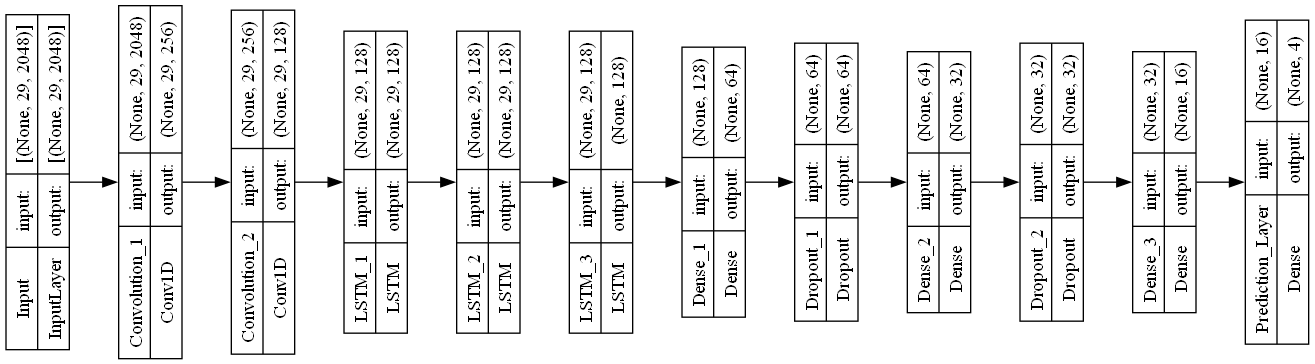
\includegraphics[width=0.9\textwidth]{model architectures/1 architecture.png}
\caption[Experiment 1 architecture]{Experiment 1 architecture. This depicts two 1D convolution layers, followed by three \acrshort{lstm} layers and then a set of dense layers with some dropout. The ``None" above refers to the batch size. Models are trained with batches of data which contain several samples of data. The 29 refers to the number of frames expected by the model. The final number for each layer is that layer's size.}
\label{fig:1 architecture}
\end{figure}
The first experiment used a basic model architecture as a basis to improve upon. The model architecture used, as shown in Figure~\ref{fig:1 architecture}, began with an input layer\footnote{\url{https://www.tensorflow.org/api_docs/python/tf/keras/layers/InputLayer}} to automatically configure the input shape accepted by the model. Two 1D convolutional\footnote{\url{https://keras.io/api/layers/convolution_layers/}} and three unidirectional \acrshort{lstm} layers\footnote{\url{https://keras.io/api/layers/recurrent_layers/lstm/}} followed this. Finally a series of dense\footnote{\url{https://keras.io/api/layers/core_layers/dense/}} and dropout layers\footnote{\url{https://keras.io/api/layers/regularization_layers/dropout/}} were employed before a prediction layer output the probabilities of the input sample belonging to each of the different classes within the dataset.\\
This architecture was inspired by Chung et al.~\cite{Lip-Reading-In-The-Wild} who suggested extending their architecture of \acrshort{cnn} to additionally include \acrshort{lstm} units.\\
1D convolution was used here as the input data only consisted of image feature vectors of the size (1, 2048). ReLU activation functions were used for each layer, excluding the final prediction layer which instead employed Softmax.\\
\Gls{dropout} layers were employed as a means of regularisation~\cite{regularization_for_DL, dropout_for_overfitting}, to avoid \gls{overfitting}. A value of 0.2 was used to drop 20\% of input units during training.\\
Categorical cross-entropy loss was used to train the model, outlined in Section~\ref{sec: Cross-Entropy Loss}. The classes used were the \gls{one_hot_encoding}s for the four word classes: \emph{about}, \emph{believe}, \emph{chance} and \emph{family}.\\
The model was trained for 100 epochs to allow for sufficient time for the model to capture nuances within the training data whilst maintaining a shorter training time. A batch size of 32 was used for similar reasons.\\
Finally, the Adam optimiser alone was used with a \acrshort{lr} of $1\times10^{-5}$. A very small \acrshort{lr} was used because lip reading is a very nuanced and subtle process.
\subsection{Results and Evaluation}
\begin{figure}
\centering
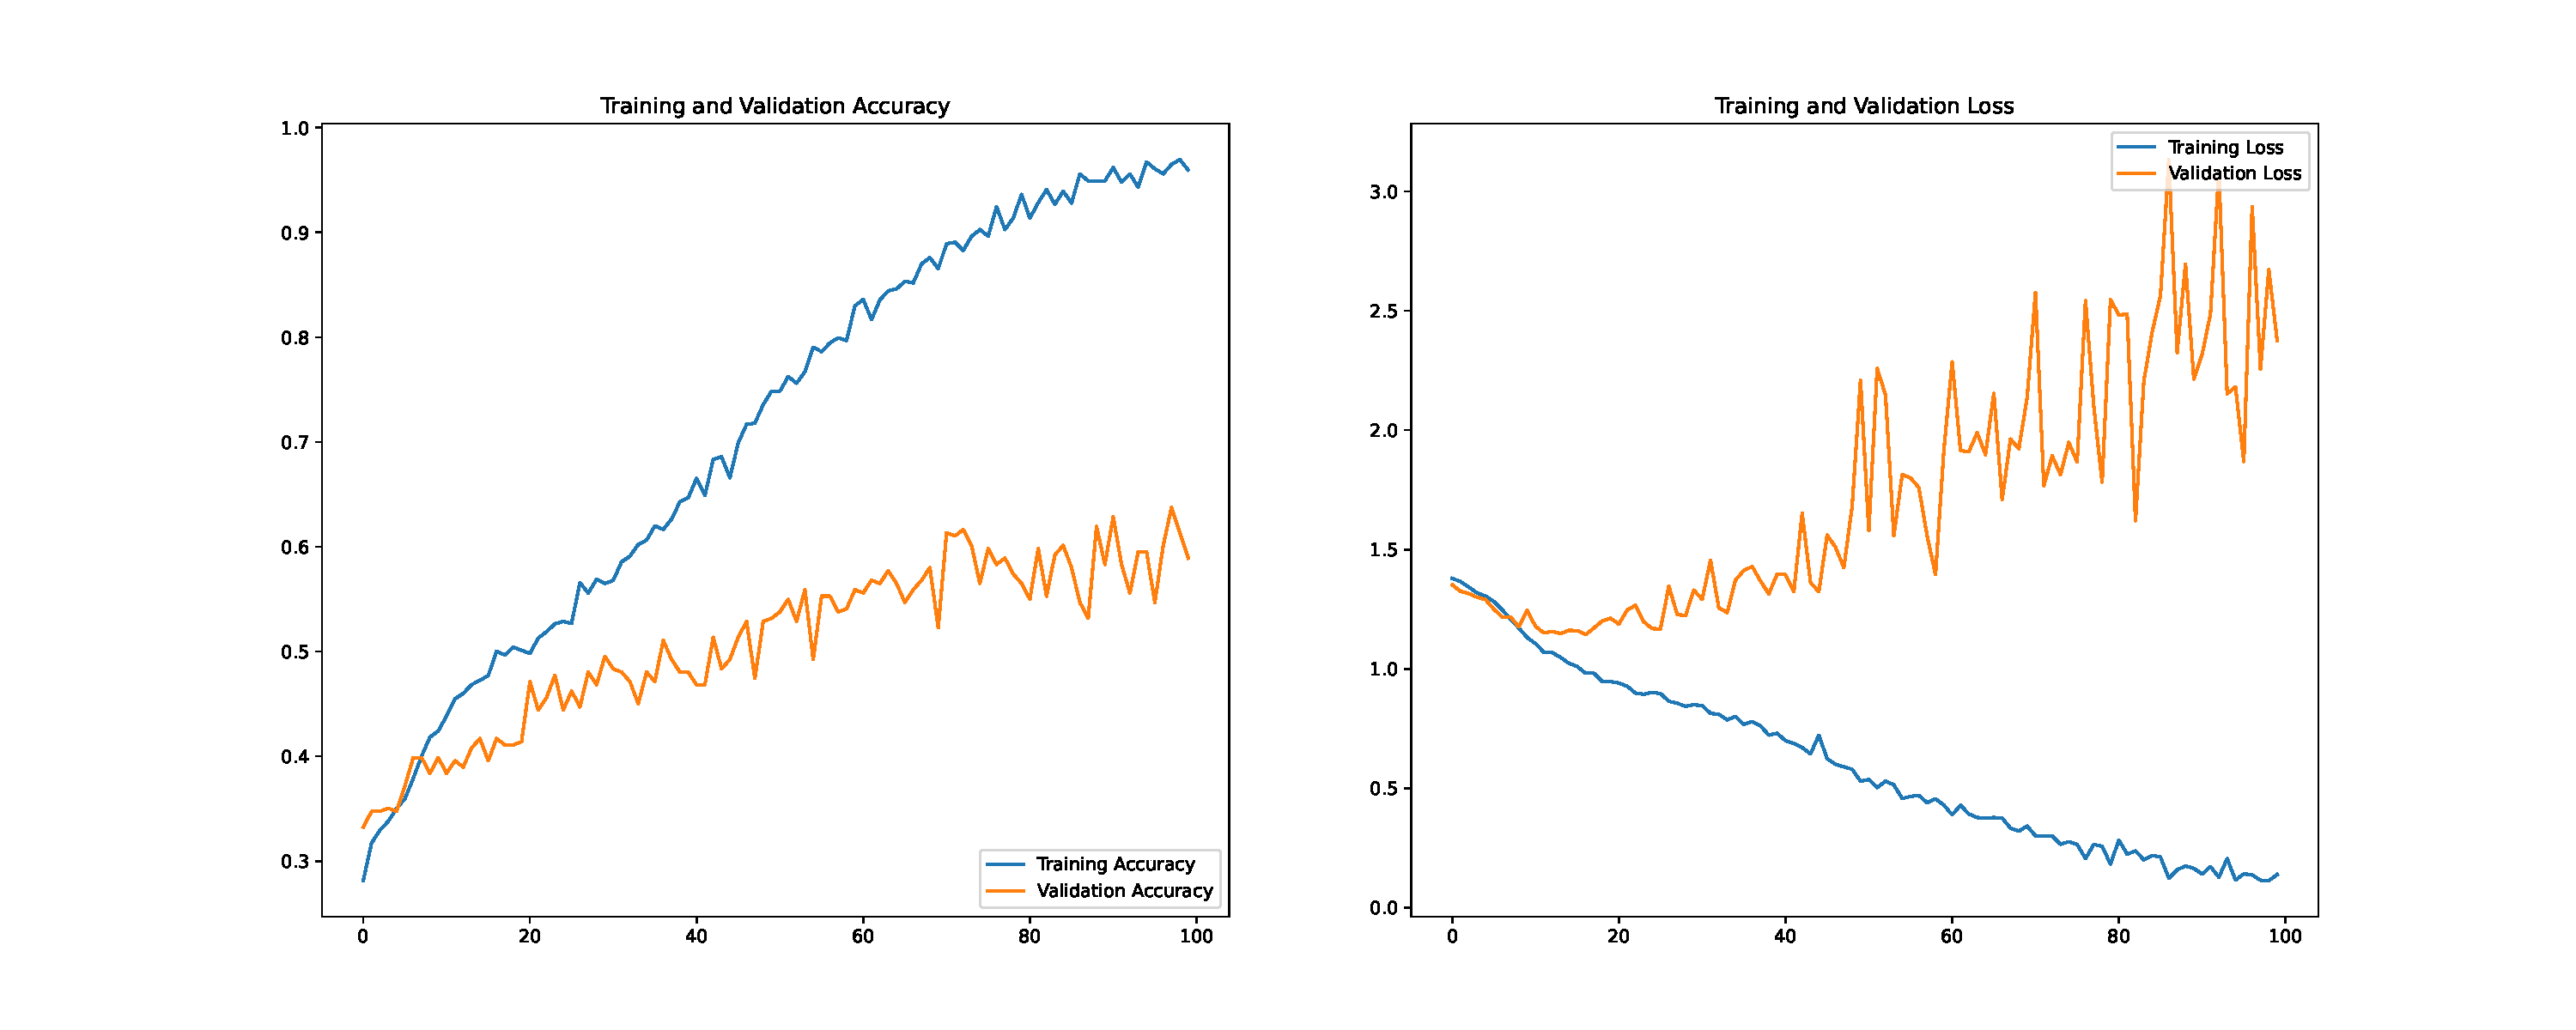
\includegraphics[width=1\textwidth]{metrics/1 metrics.pdf}
\caption[Experiment 1 results]{Experiment 1 results. This depicts training and testing accuracy and loss. Accuracy measures of the number of videos that were given the correct label of the word being spoken. Loss gives a measure of the categorical cross-entropy loss of the different predictions.}
\label{fig:1 results}
\end{figure}
\begin{table}
\centering
\begin{tabular}{|c|c|c|c|} 
 \hline
 Experiment &  Testing Accuracy & Testing Loss & \acrshort{wer} \\ [0.2ex] 
 \hline
 1 & \accuracyone & \lossone & \werone \\ 
 \hline
\end{tabular}
\caption[The testing accuracy, loss and \acrshort{wer} for experiment 1]{The testing accuracy, loss and \acrshort{wer} for experiment 1. These results were captured by running the model against a testing dataset: a dataset that was not used during training of the model.}
\label{table: 1 results}
\end{table}
The first experiment yielded promising results, as shown in Figure~\ref{fig:1 results} and Table~\ref{table: 1 results}. Clear \gls{overfitting} occurred early within training, evident by the training and testing accuracies and losses diverging early. There could be many potential causes of \gls{overfitting} such as there not being enough data, data being too noisy or the model being too complex. There are many potential ways to reduce \gls{overfitting}. These include \gls{data_augmentation}, data regularisation~\cite{regularization_for_DL, dropout_for_overfitting} or reducing the size and complexity of the model.\\
Due to the results of this experiment, the second experiment instead employed some \gls{data_augmentation} methods,  attempting to reduce noise within the data.
\section{Experiment 2: Frame Pruning}
\label{sec: Experiment 2}
% Experiment 3
% Added frame pruning & data_augmentation
\subsection{Model Architecture}
The same model architecture was used as in Section~\ref{sec: Experiment 1}. However, further data preprocessing was carried out before training, aiming to reduce \gls{overfitting}.\\
As outlined within Section~\ref{sec: LRW Dataset}, the structure of \gls{lrw} are 29 frame videos that contain multiple word utterances. Only the primary word utterances (\emph{about}, \emph{believe}, \emph{chance} or \emph{family}) within each video are labelled. Whilst this can be beneficial, this could result in \gls{overfitting}. This is because the model might fixate on commonly occurring words around the primary word, such as ``I believe" rather than ``believe". This could cause \gls{underfitting} if the data samples are too noisy, resulting in difficulty converging to a valid solution.\\
This experiment employed two methods to overcome \gls{overfitting} encountered within Section~\ref{sec: Experiment 1}: frame pruning and \gls{data_augmentation}.\\
Frame pruning was used to remove frames from the start and end of video data samples, focusing more on the central part of the video and thus the primary word utterance. This could reduce \gls{overfitting} as there is less noise present in the data.\\
The downside of frame pruning is that it could introduce \gls{underfitting} or worsen the performance of models. Indiscriminate removal of frames could remove intrinsic information from each data sample.\\
The method used for \gls{data_augmentation} was horizontal flipping. The frames for each video were horizontally flipped, and these new samples were added to the dataset. This had the effect of doubling the amount of data available for training, validation and testing. This method was used as it is one of the easiest \gls{data_augmentation} methods to implement~\cite{og_data_augmentation} whilst still creating diverse enough data.\\
The downside of this \gls{data_augmentation} method is that it could lead to \gls{overfitting}. After \gls{data_augmentation} there will be two copies of every \gls{lrw} sentence, possibly worsening the issue of noisy words. If the model has even more samples of ``I believe" it may become even more focused on the noisy ``I", regardless of frame flipping. This data augmentation method will preserve the structure of sentences; whilst the data might visually be different, it is not semantically diverse\\
Only 50 epochs were carried out for this training run, to conserve computational power. \Gls{overfitting} occurred early within the first training run and thus a high epoch number was not required to observe a similar result.
\subsection{Results and Evaluation}
\begin{figure}
\centering
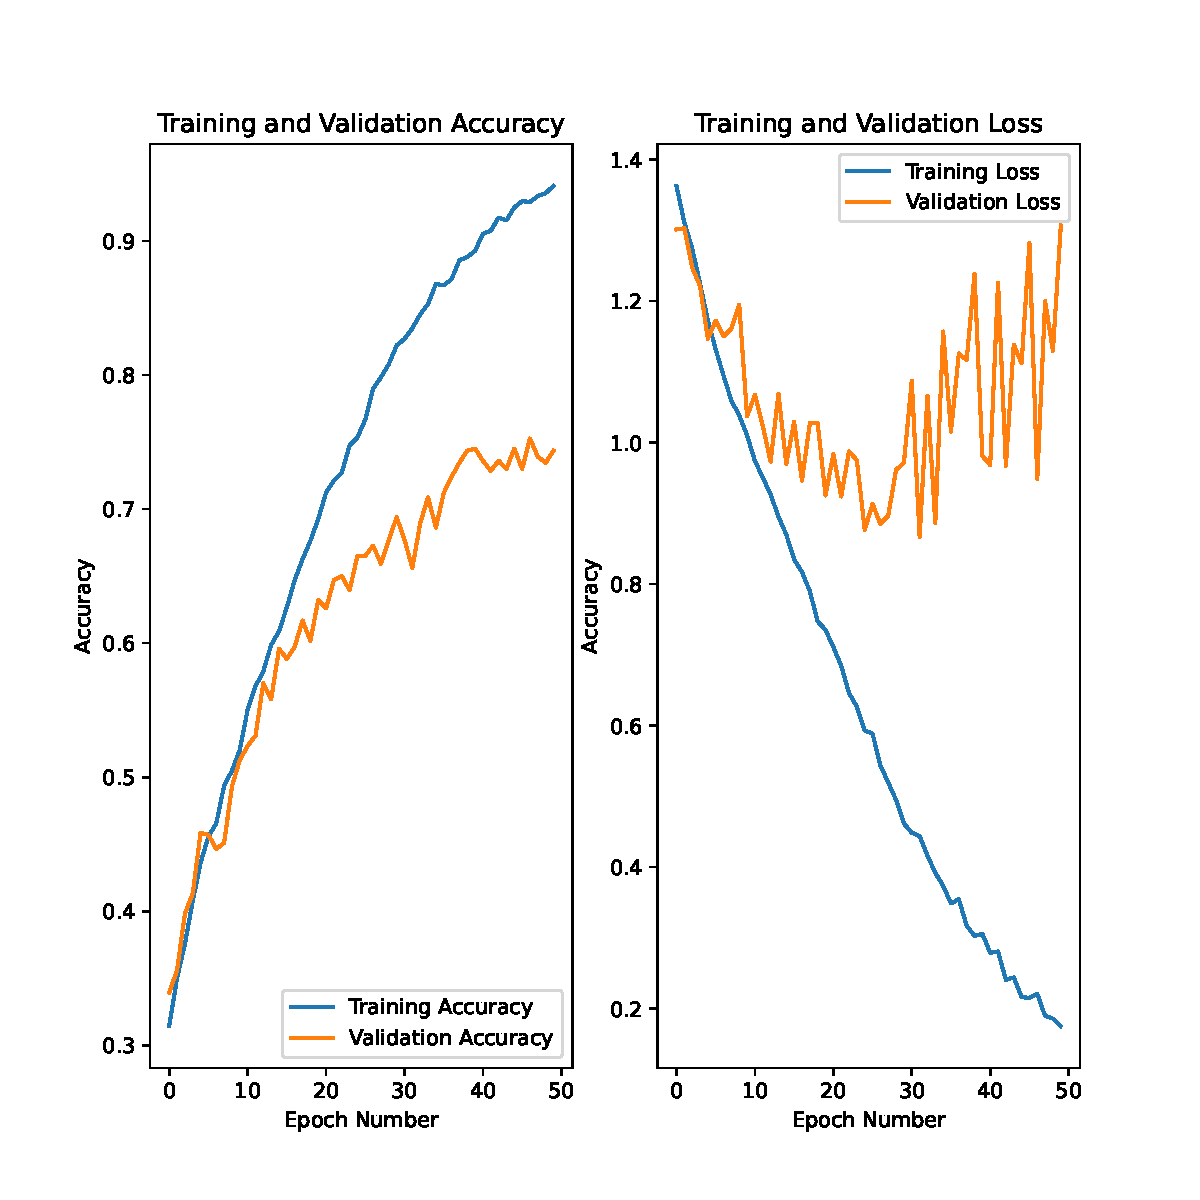
\includegraphics[width=0.5\textwidth]{metrics/2 metrics.pdf}
\caption[Experiment 2 results]{Experiment 2 results. This shows the effect of adding frame pruning and \gls{data_augmentation}.}
\label{fig:2 results}
\end{figure}
\begin{table}
\centering
\begin{tabular}{|c|c|c|c|} 
 \hline
 Experiment &  Testing Accuracy & Testing Loss & \acrshort{wer} \\ [0.2ex] 
 \hline
 2 & \accuracytwo & \losstwo & \wertwo \\ 
 \hline
\end{tabular}
\caption{The testing accuracy, loss and \acrshort{wer} for experiment 2.}
\label{table: 2 results}
\end{table}
As shown in Figure~\ref{fig:2 results} and Table~\ref{table: 2 results}, this model performed better than the previous experiment. Early stopping helped to reduce the effect of \gls{overfitting} and improve the accuracy of the model.\\
In conclusion, frame pruning and \gls{data_augmentation} did benefit the process; however, \gls{overfitting} was still occurring.
\section{Experiment 3: Bidirectional LSTM Architecture}
\label{sec: Experiment 3}
% Experiment 7
% Bi-lstm
\subsection{Model Architecture}
\begin{figure}
\centering
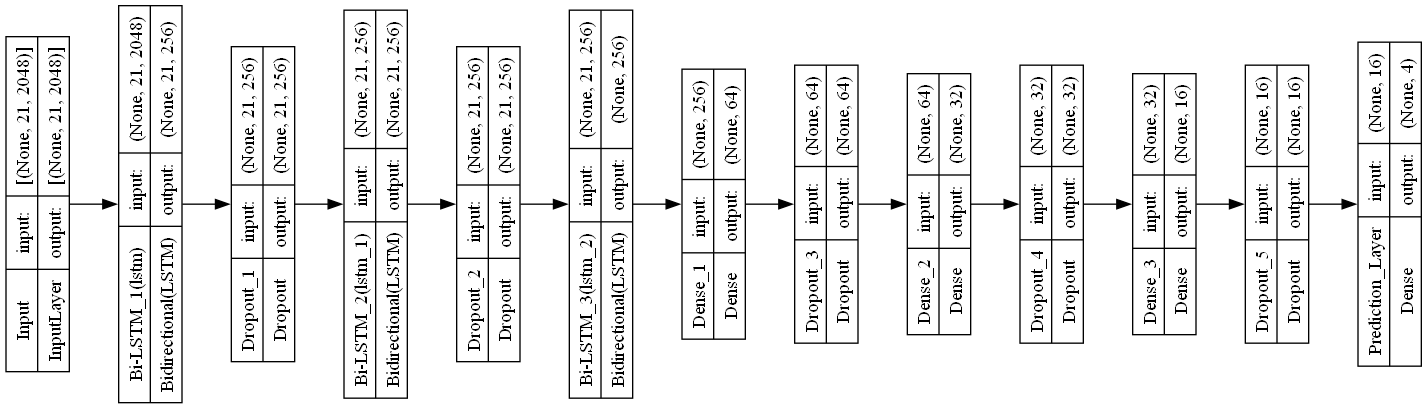
\includegraphics[width=0.9\textwidth]{model architectures/3 architecture.png}
\caption[Experiment 3 architecture]{Experiment 3 architecture. This depicts the \acrshort{bilstm} architecture employed for lip reading. The model took visual feature vectors as input to a series of \acrshort{bilstm} layers. \Gls{dropout} was employed after each layer to reduce the effect of \gls{overfitting}. ReLU activation functions were utilised for each layer except the final which employed Softmax.}
\label{fig:3 architecture}
\end{figure}
For this experiment, a different model architecture was investigated (see Figure~\ref{fig:3 architecture}). Rather than a \acrshort{cnn} combined with an \acrshort{lstm}, a pure \acrshort{bilstm}\footnote{\url{https://keras.io/api/layers/recurrent_layers/bidirectional/}} architecture was studied.\\
Typically, convolution is utilised for image or video data (2D or 3D data) to reduce the dimensionality of the data and looking at the relationship between image regions. However, for this experiment we have already employed a visual feature extractor, effectively skipping this step.\\
In the previous experiment, only unidirectional \acrshort{lstm} layers were utilised. Instead in this experiment, we employed \acrshort{bilstm} layers to capture both left and right context within the videos.\\
Training lasted for 150 epochs, allowing the model more time to train and learn the data since a simple model was being investigated. Otherwise, the details of this experiment (\acrshort{lr}, early stopping, loss, etc) remained the same as the previous one. The same activation functions of ReLU were employed within the \acrshort{bilstm} layers.
\subsection{Results and Evaluation}
\begin{figure}
\centering
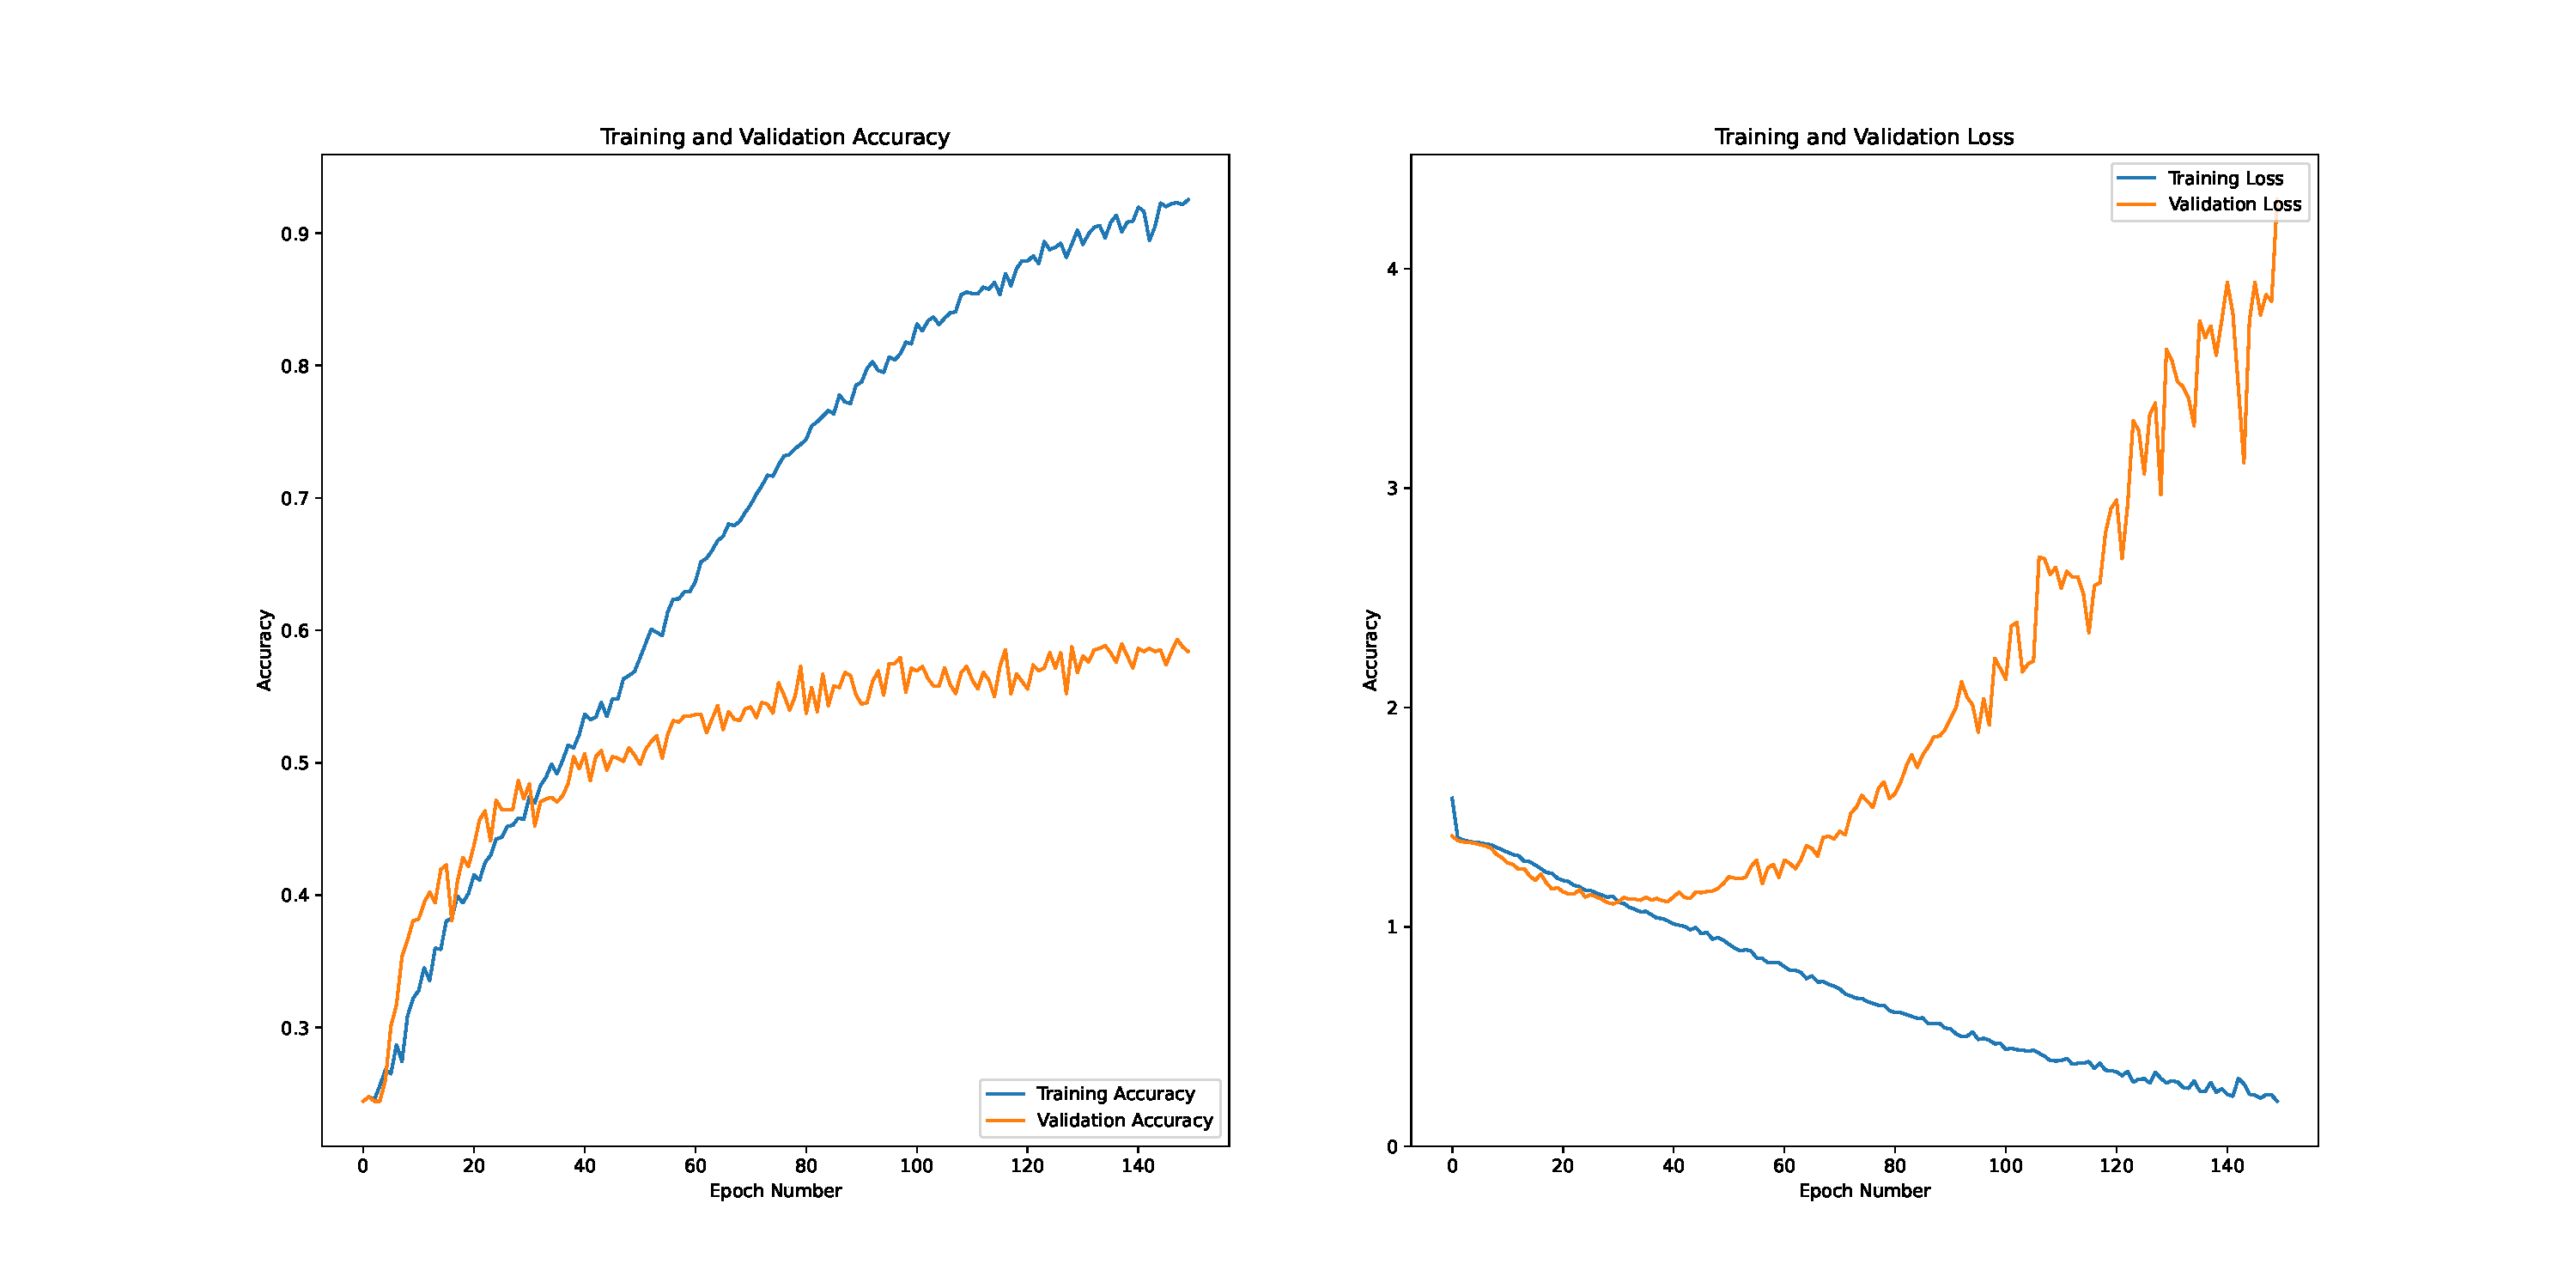
\includegraphics[width=1\textwidth]{metrics/3 metrics.pdf}
\caption[Experiment 3 results]{Experiment 3 results.}
\label{fig:3 results}
\end{figure}
\begin{table}
\centering
\begin{tabular}{|c|c|c|c|} 
 \hline
 Experiment &  Testing Accuracy & Testing Loss & \acrshort{wer} \\ [0.2ex] 
 \hline
 3 & \accuracythree & \lossthree & \werthree \\ 
 \hline
\end{tabular}
\caption{The testing accuracy, loss and \acrshort{wer} for experiment 3.}
\label{table: 3 results}
\end{table}
As shown in Figure~\ref{fig:3 results} and Table~\ref{table: 3 results}, this architecture actually performed worse than the previous models.\\
The maximum accuracy and minimum loss achieved were both lower than the models trained in the first and second experiments. However, \gls{overfitting} occurred later in training, giving promising results for this architecture.\\
Further experimentation was conducted on this architecture aiming to produce better results.
\section{Experiment 4: Manual Adaptive Learning Rate}
\label{sec: Experiment 4}
% Experiment 8
% Adaptive learning rate
\subsection{Model Architecture}
For this experiment, the same model architecture was used as in Section~\ref{sec: Experiment 3}; however, the \acrshort{lr} was changed.\\
Previously the Adam optimiser on its own had been employed to varying success. Instead, as mentioned in Section~\ref{sec: Learning Rate}, a combination of both the Adam optimiser and another \acrshort{lr} scheduling method is beneficial and thus was applied. For this experiment, Adam was used to control the \acrshort{lr} of parameters more precisely but the \acrshort{lr} was also altered manually.\\
Three primary experiments were carried out. In each, after 20 epochs the \acrshort{lr} was multiplied by a decimal value. The values used for the experiments were 0.9, 0.5 and 0.7.\\
A higher initial \acrshort{lr} of $1\times10^{-4}$ was used, compared with previous experiments. In most cases, a larger \acrshort{lr} should be used initially, decreasing this over time~\cite{batch-size-on-the-generalizability}. A large initial \acrshort{lr} allows the model to find the global minimum in the loss and then converge quickly as the \acrshort{lr} decreases.
\subsection{Results and Evaluation}
\begin{figure}
\centering
    \subfloat[\centering Experiment 4.1. \acrshort{lr} multiplier equals 0.9.]{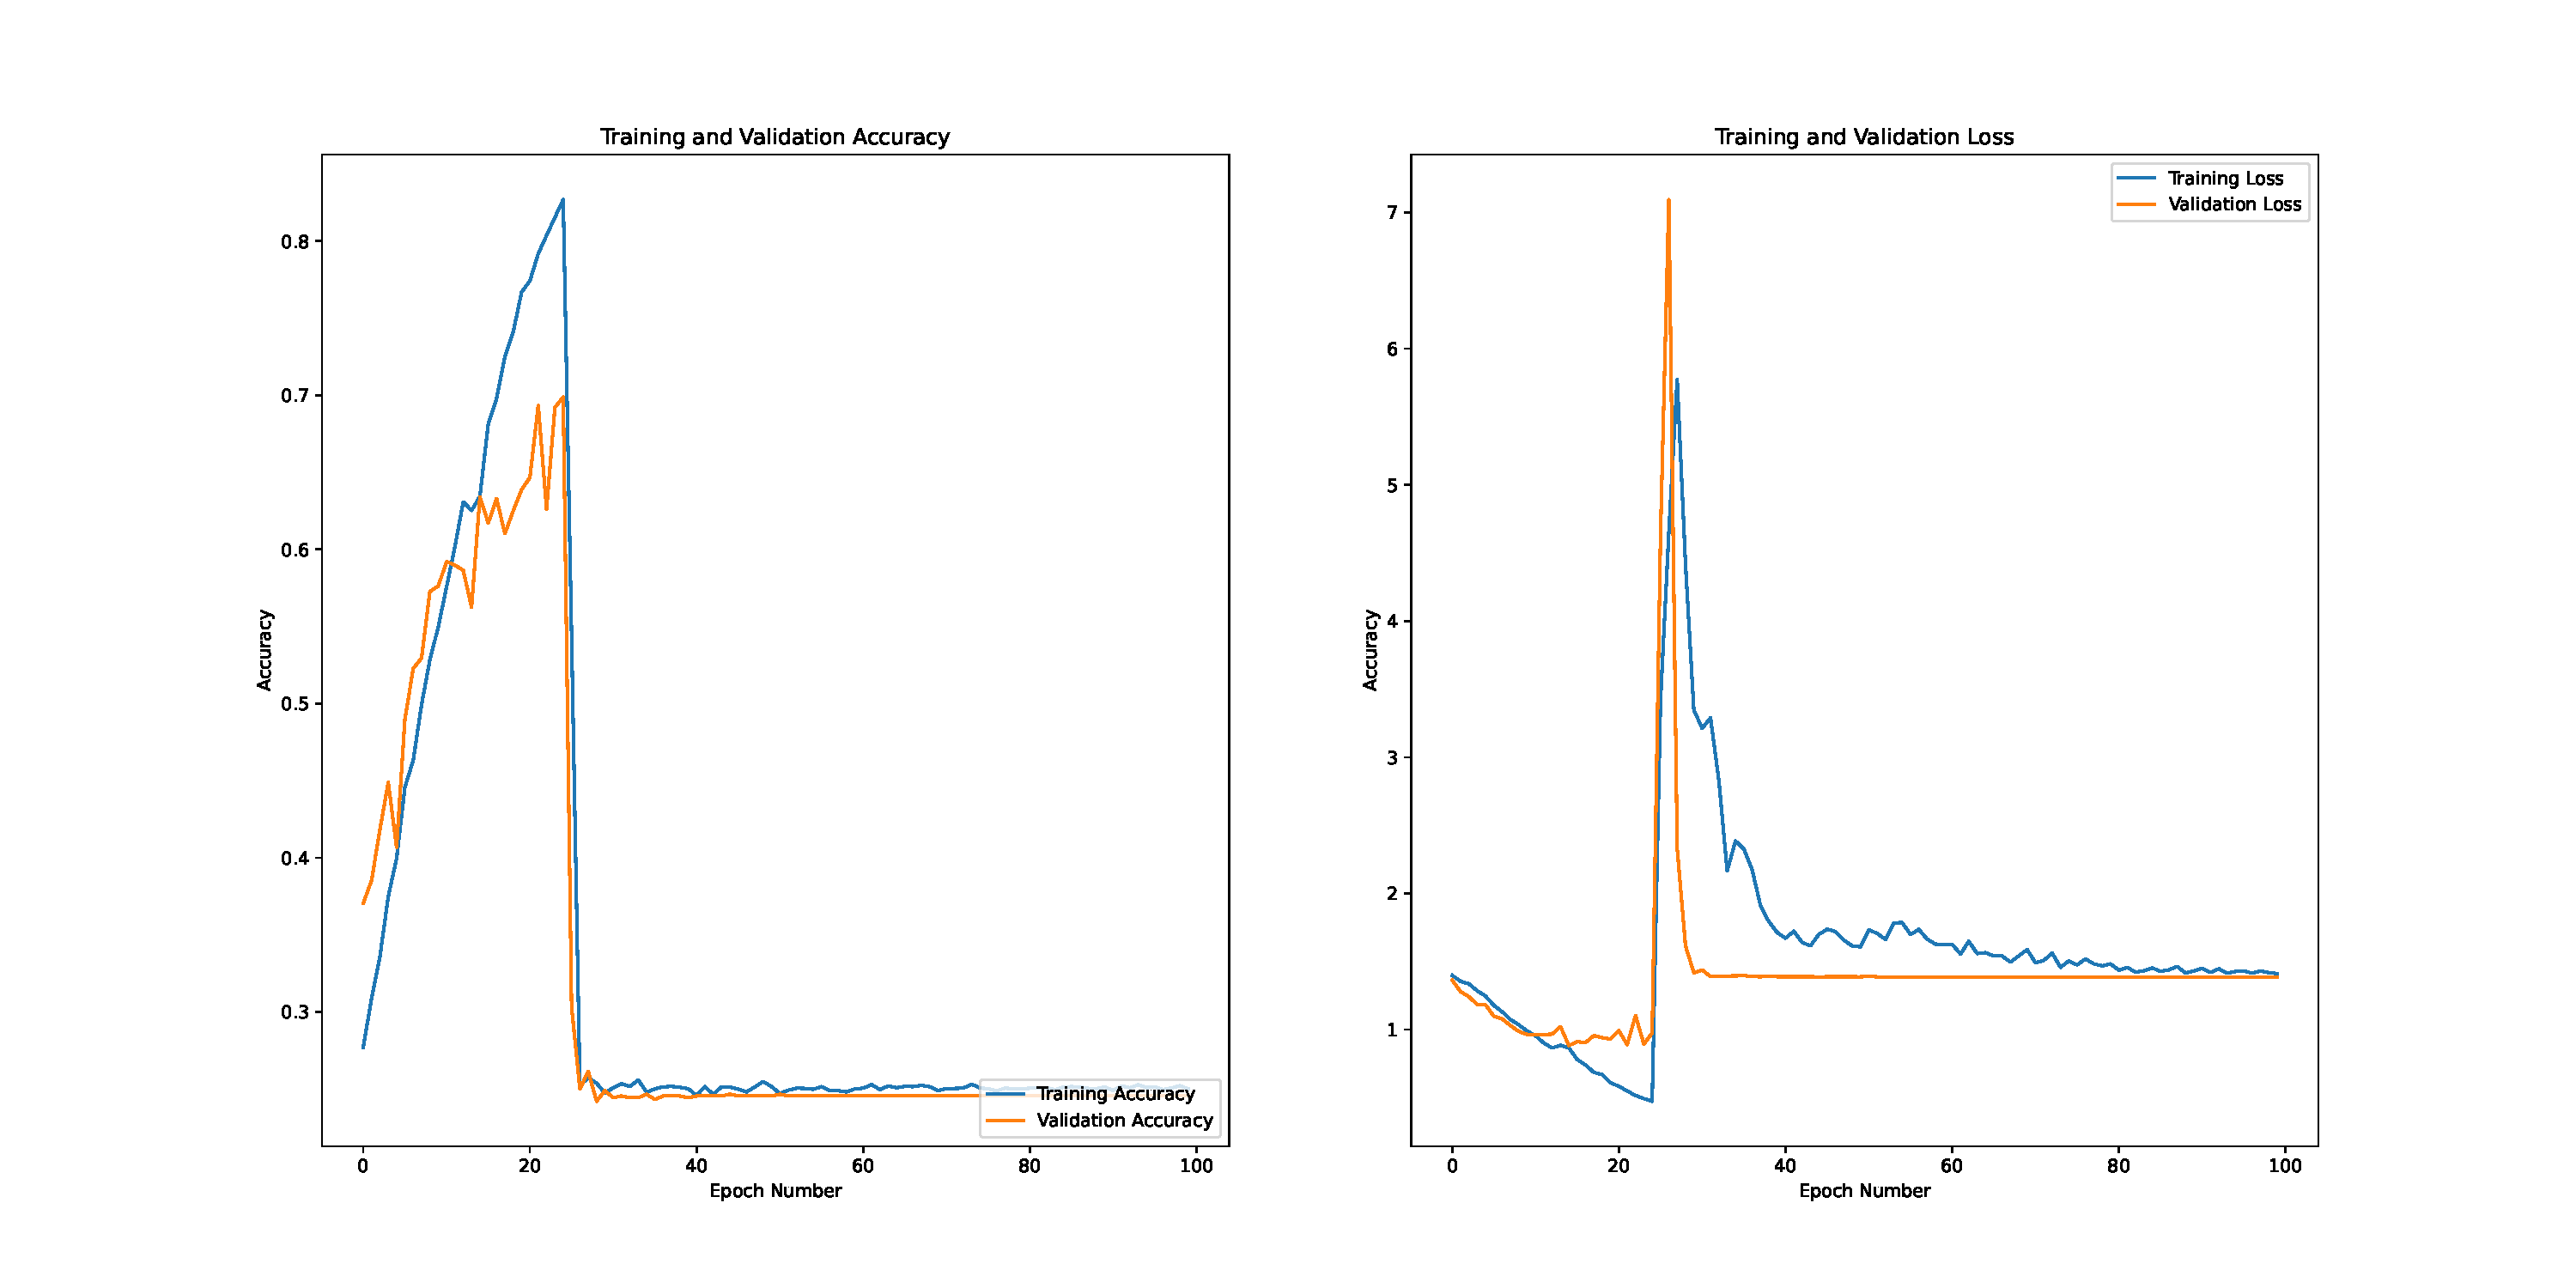
\includegraphics[width=0.5\textwidth]{metrics/4.1 metrics.pdf}}
    \subfloat[\centering Experiment 4.2. \acrshort{lr} multiplier equals 0.5.]{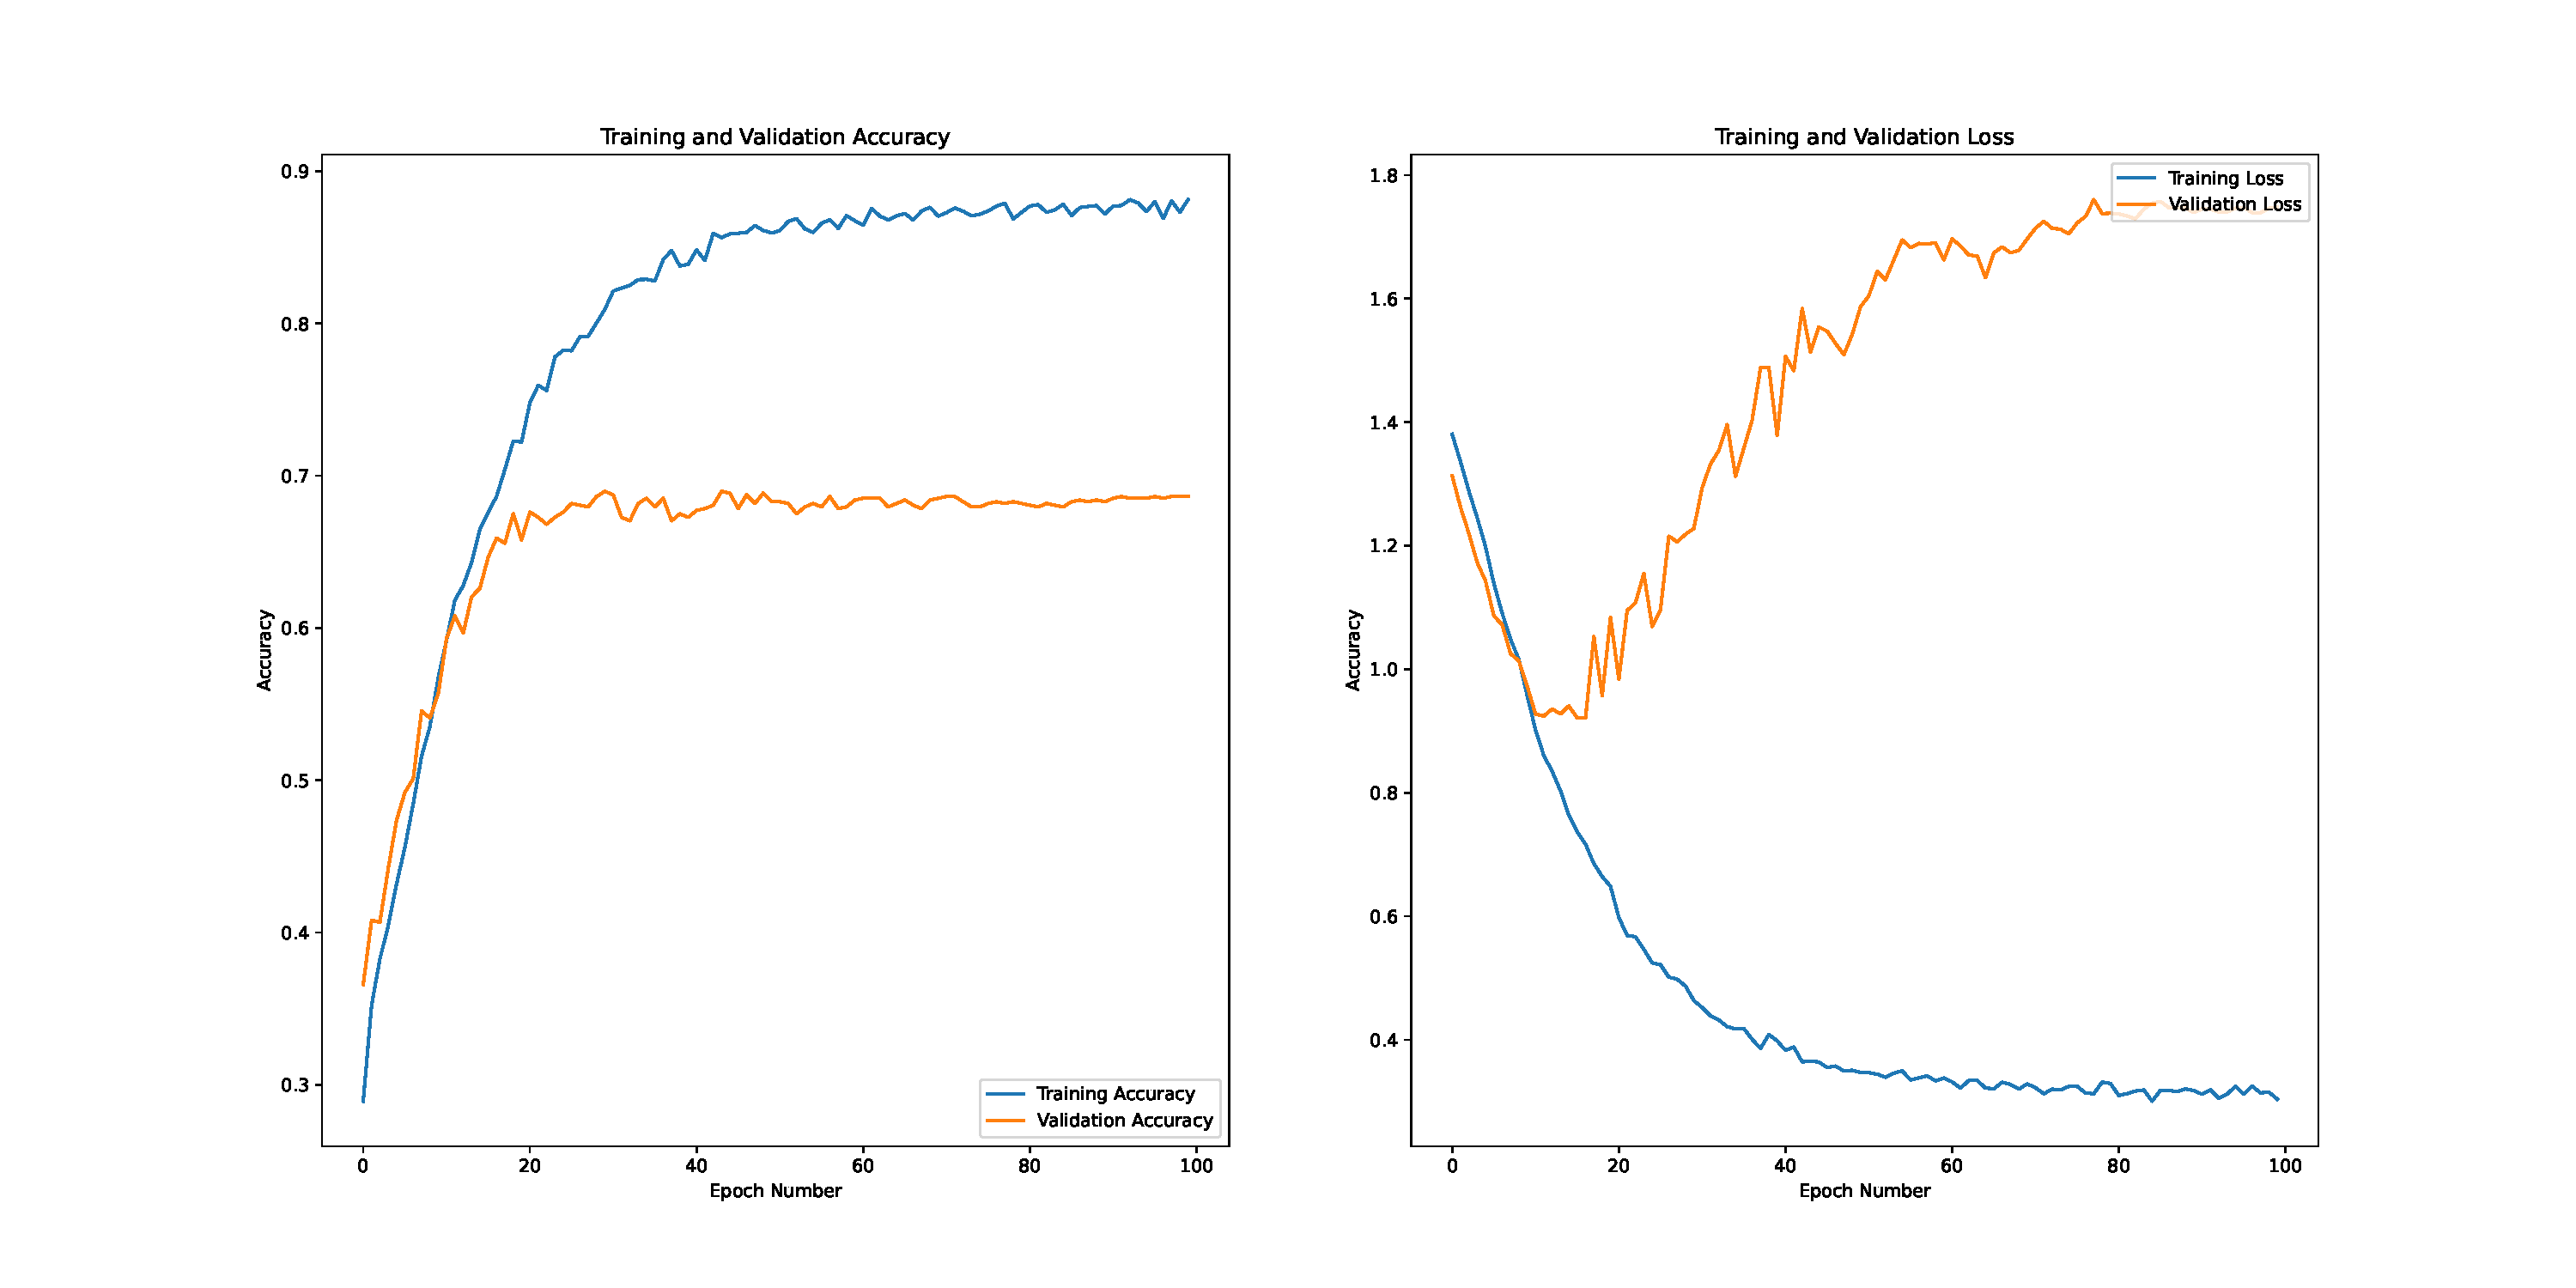
\includegraphics[width=0.5\textwidth]{metrics/4.2 metrics.pdf}}\\
    \subfloat[\centering Experiment 4.3. \acrshort{lr} multiplier equals 0.7.]{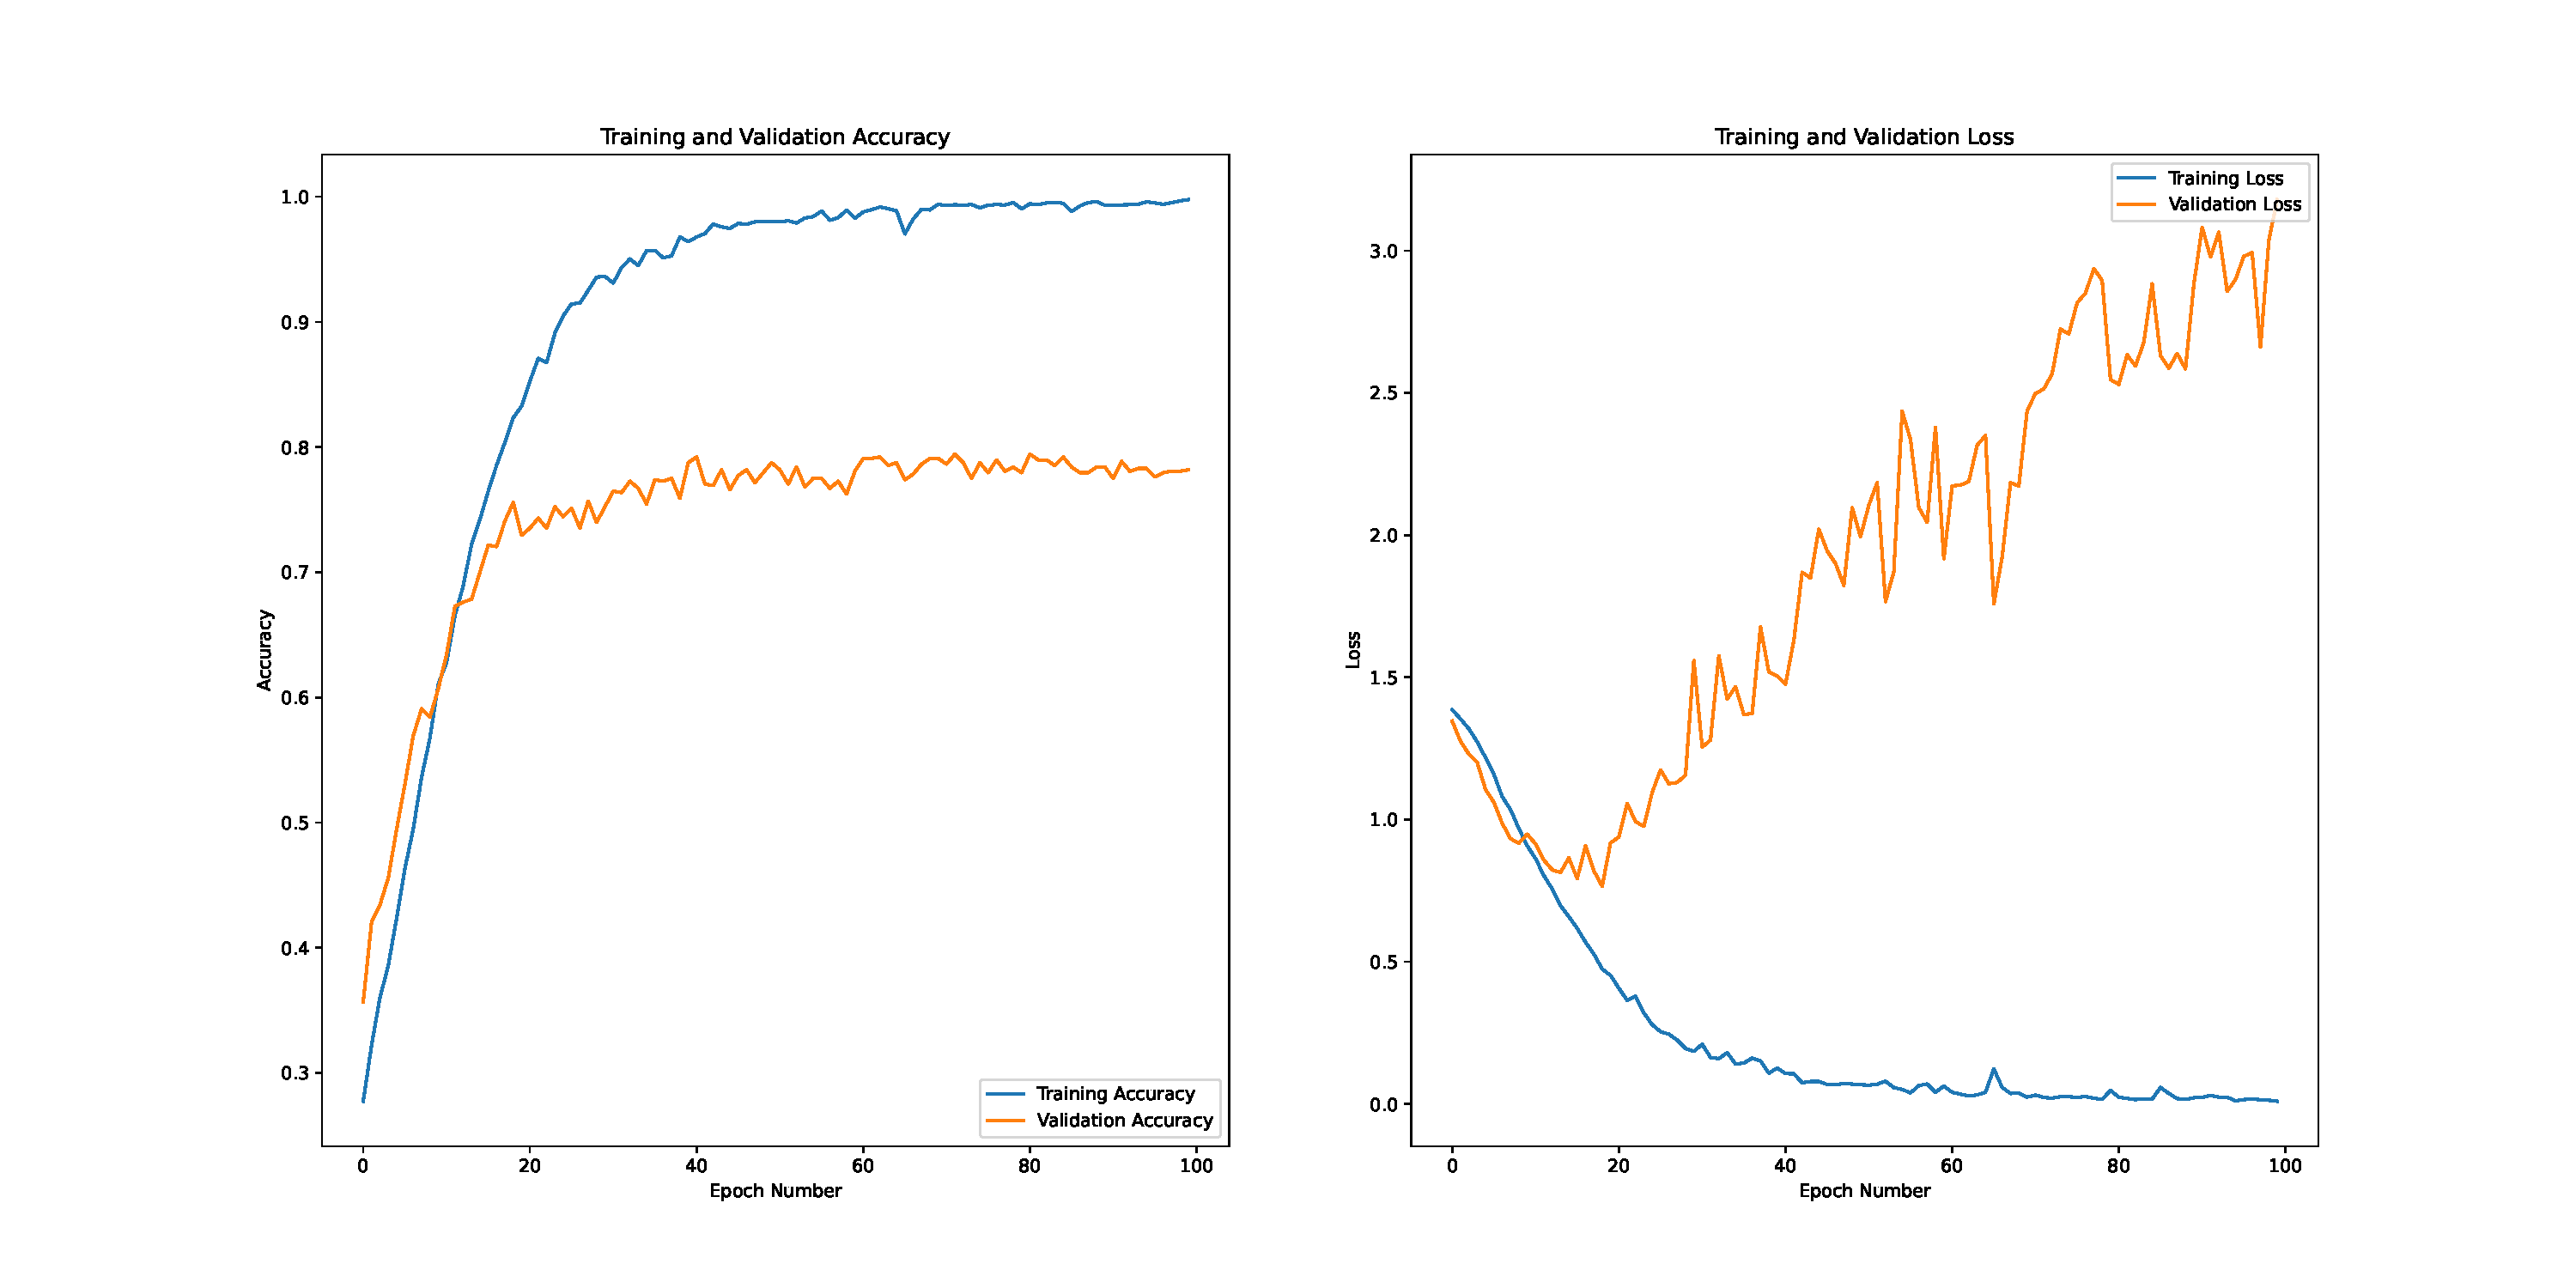
\includegraphics[width=0.5\textwidth]{metrics/4.3 metrics.pdf}}
\caption[Experiment 4 results]{Experiment 4 results. This depicts the three experiments with adaptive \acrshort{lr} via the Adam optimiser combined with a manual \acrshort{lr} change via a multiplier. All three experiments used an initial \acrshort{lr} of 0.0001 and multiplied the \acrshort{lr} every 20 epochs. Experiment 4.1 used a decay rate of 0.9, 4.2 used 0.5 and 4.3 used 0.7.}
\label{fig:4 results}
\end{figure}
\begin{table}
\centering
\begin{tabular}{|c|c|c|c|} 
 \hline
 Experiment &  Testing Accuracy & Testing Loss  & \acrshort{wer} \\ [0.2ex] 
 \hline
 4.1 & \accuracyfourone & \lossfourone & \werfourone \\
 4.2 & \accuracyfourtwo & \lossfourtwo & \werfourtwo \\
 4.3 & \accuracyfourthree & \lossfourthree & \werfourthree \\
 \hline
\end{tabular}
\caption{The testing accuracy, loss and \acrshort{wer} for experiment 4.}
\label{table: 4 results}
\end{table}
The results of the adaptive \acrshort{lr} experiment, represented in Figure~\ref{fig:4 results} and Table~\ref{table: 4 results}, show that altering the \acrshort{lr} significantly impacts the performance of models. The same model architecture but a different \acrshort{lr} scheduling method resulted in a much-improved model, as compared with Section~\ref{sec: Experiment 3} which just used the Adam optimiser.\\
The initial experiment, which employed 0.9 for the \acrshort{lr} multiplier, had an interesting performance. There is a large dip in performance where the model diverged and left the local minimum in the loss. The \acrshort{lr} was potentially changed too fast in this case.\\
A \acrshort{lr} multiplier of 0.5 reduced this effect, causing some \gls{overfitting} but not model divergence. Moreover, the accuracy and loss with this architecture spiked far less than with previous experiments and the testing metrics gave the best results seen yet.\\
A \acrshort{lr} multiplier of 0.7 strangely did not represent a middle-ground between the two experiments but instead a dip in performance. Because of this, the multiplier of 0.5 was applied to further experimentation.
\section{Experiment 5: Lip Landmarks}
\label{sec: Experiment 5}
% Experiment 8
% Only lip landmarks
\subsection{Model Architecture}
\begin{figure}
\centering
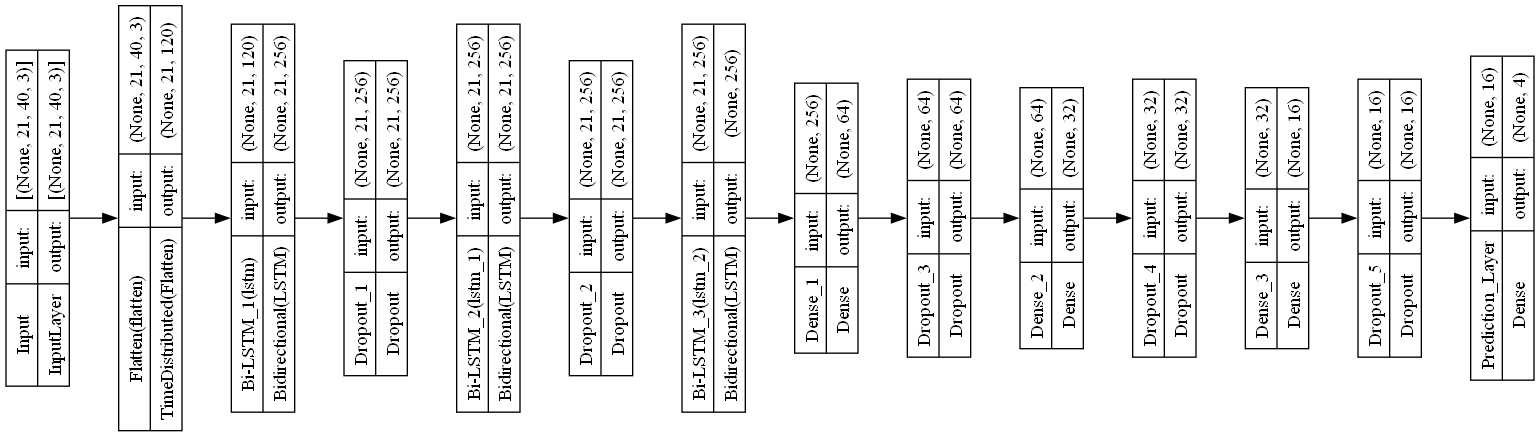
\includegraphics[width=0.9\textwidth]{model architectures/5 architecture.png}
\caption{Experiment 5 architecture.}
\label{fig:5 architecture}
\end{figure}
Previously, only visual features had been used for training. Alternatively, this experiment investigated the use of only landmark features as a model input.\\
As shown in Figure~\ref{fig:5 architecture}, the same model architecture was used as Section~\ref{sec: Experiment 4} except that the input size of the model was changed. Rather than accepting 2048 long feature vectors, the model had an input size of 120. This was formed of the 40 lip landmarks, represented with $(X, Y, Z)$ coordinates, as specified in Section~\ref{sec: Landmark Feature Extraction}.\\
Similarly to Section~\ref{sec: Experiment 4}, a set of sub-experiments were carried out to find the optimal performance of this architecture. The same model was used initially, to better compared with the previous experiment. The \acrshort{lr} was then altered to find optimal performance.\\
Various methods were utilised to schedule and vary the \acrshort{lr} throughout training. Whilst manual \acrshort{lr} scheduling had already been investigated, other settings were trialled. The Adam optimiser was employed for each experiment.\\
Experiment~5.1 used the same \acrshort{lr} scheduling as in experiment~4.2. Experiments~5.2 to 5.4 used different, manual \acrshort{lr} scheduling methods and 5.5 used exponential decay, as explained in Section~\ref{sec: Learning Rate}. Keras' exponential decay\footnote{\url{https://keras.io/api/optimizers/learning_rate_schedules/exponential_decay/}} was used to implement the decay method.
\subsection{Results and Evaluation}
\begin{figure}
\centering
    \subfloat[\centering Experiment 5.1.]{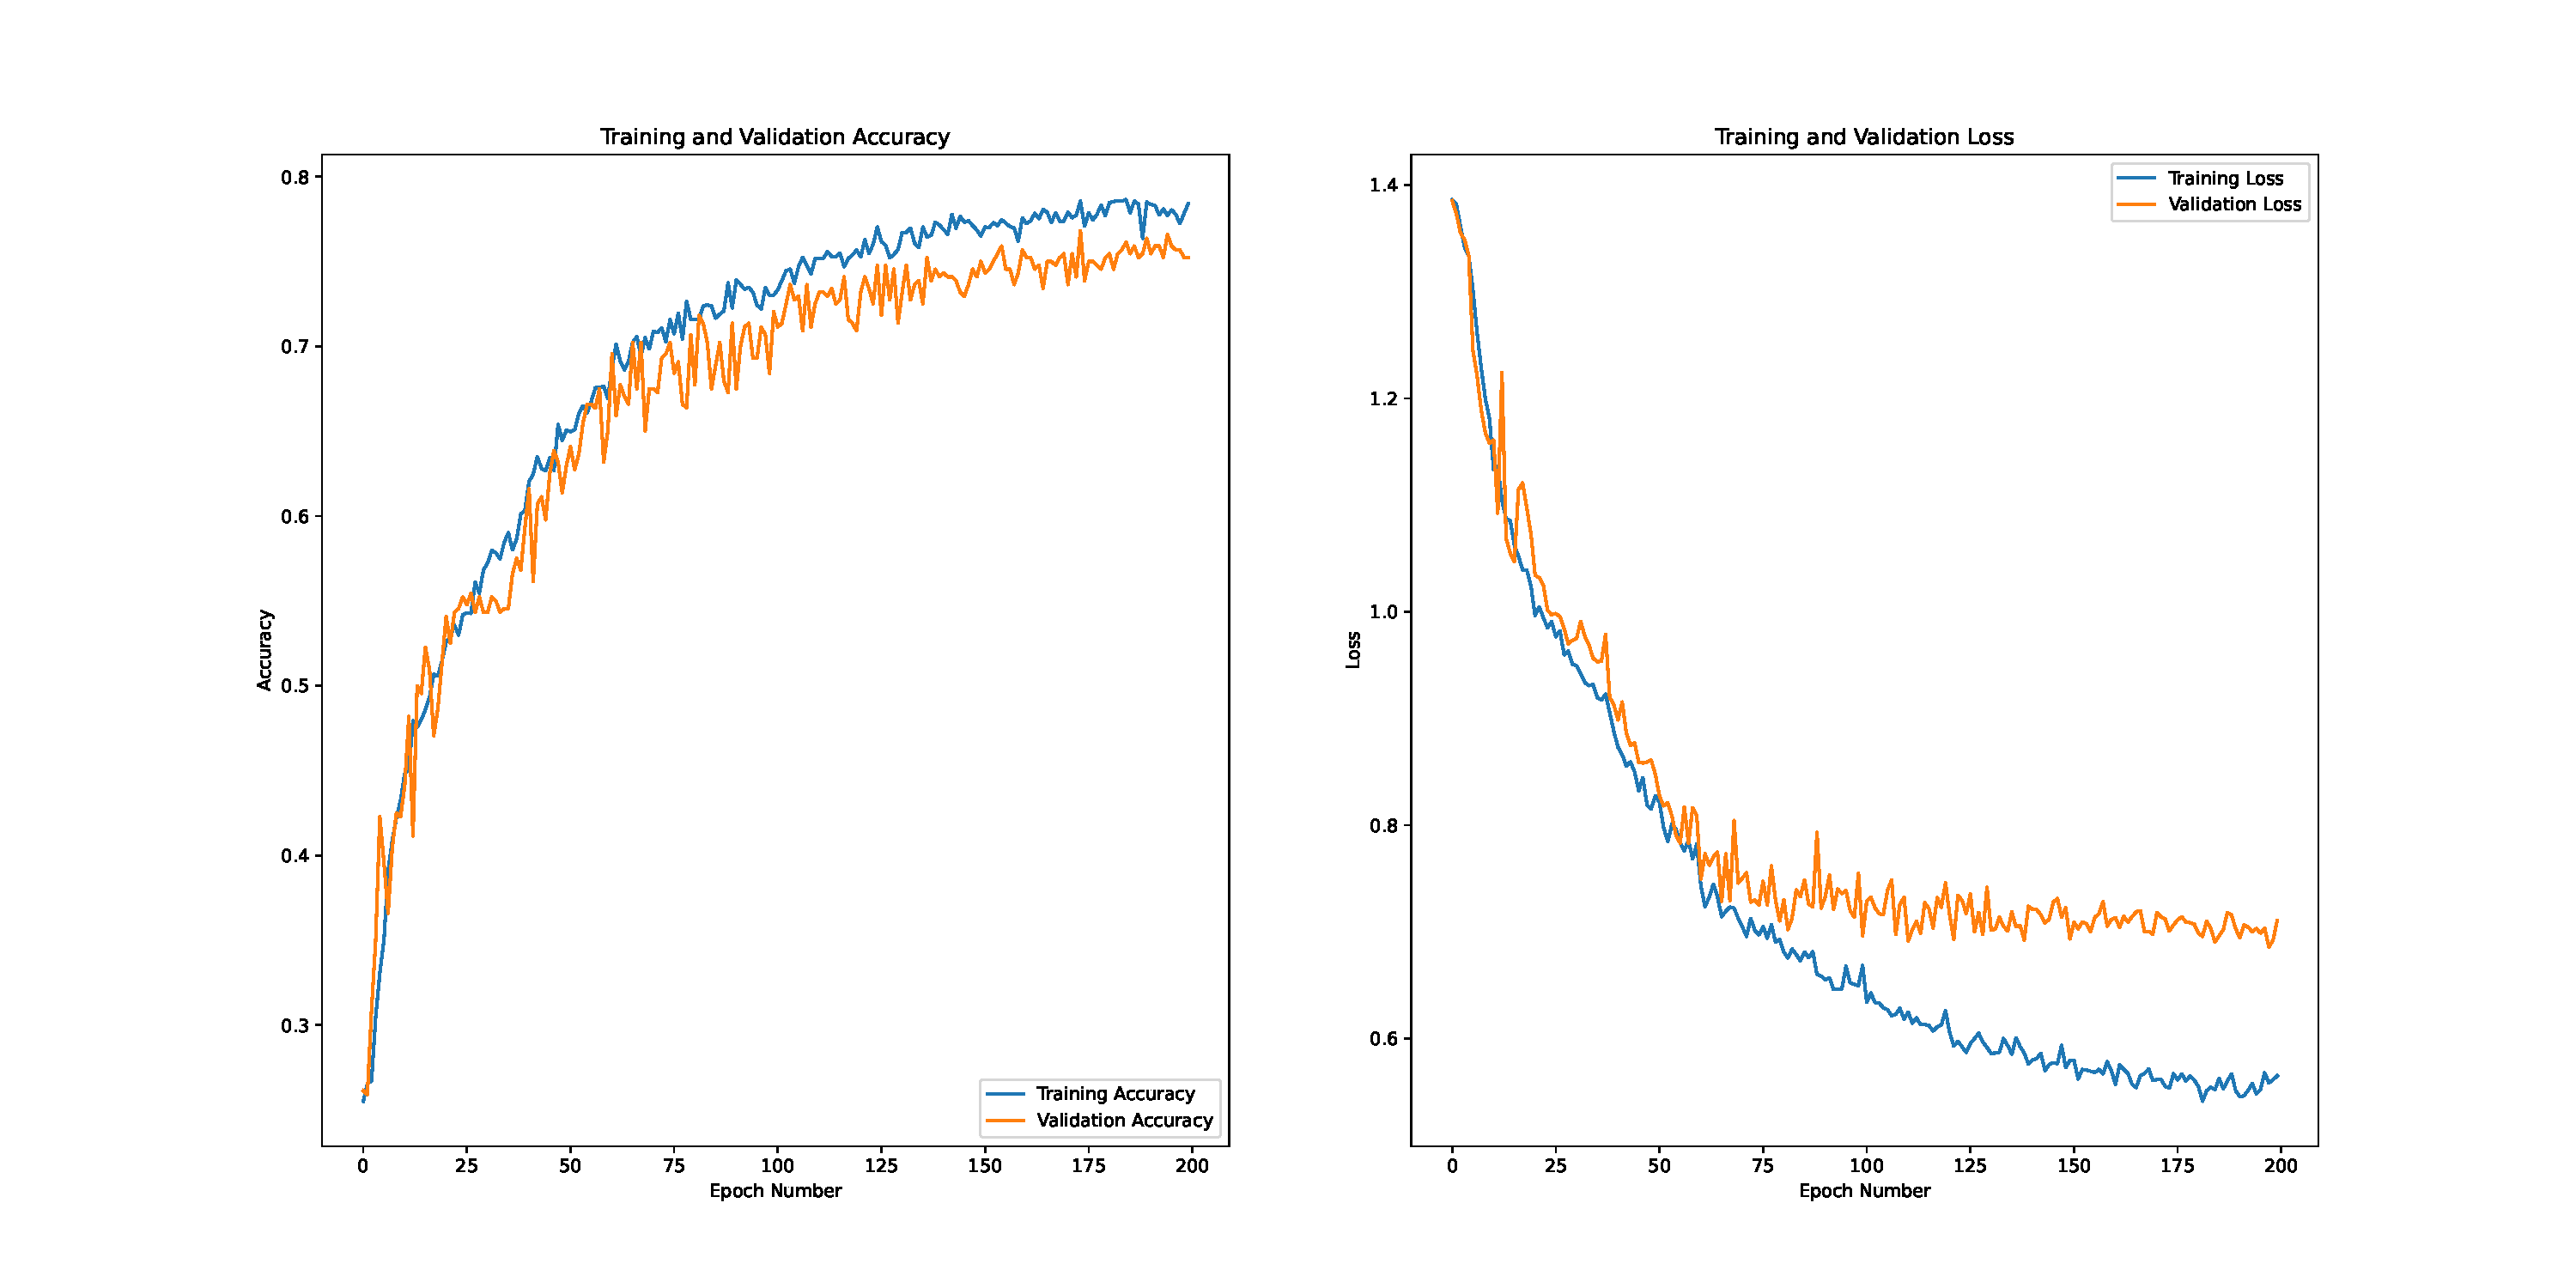
\includegraphics[width=0.5\textwidth]{metrics/5.1 metrics.pdf}}
    \subfloat[\centering Experiment 5.2.]{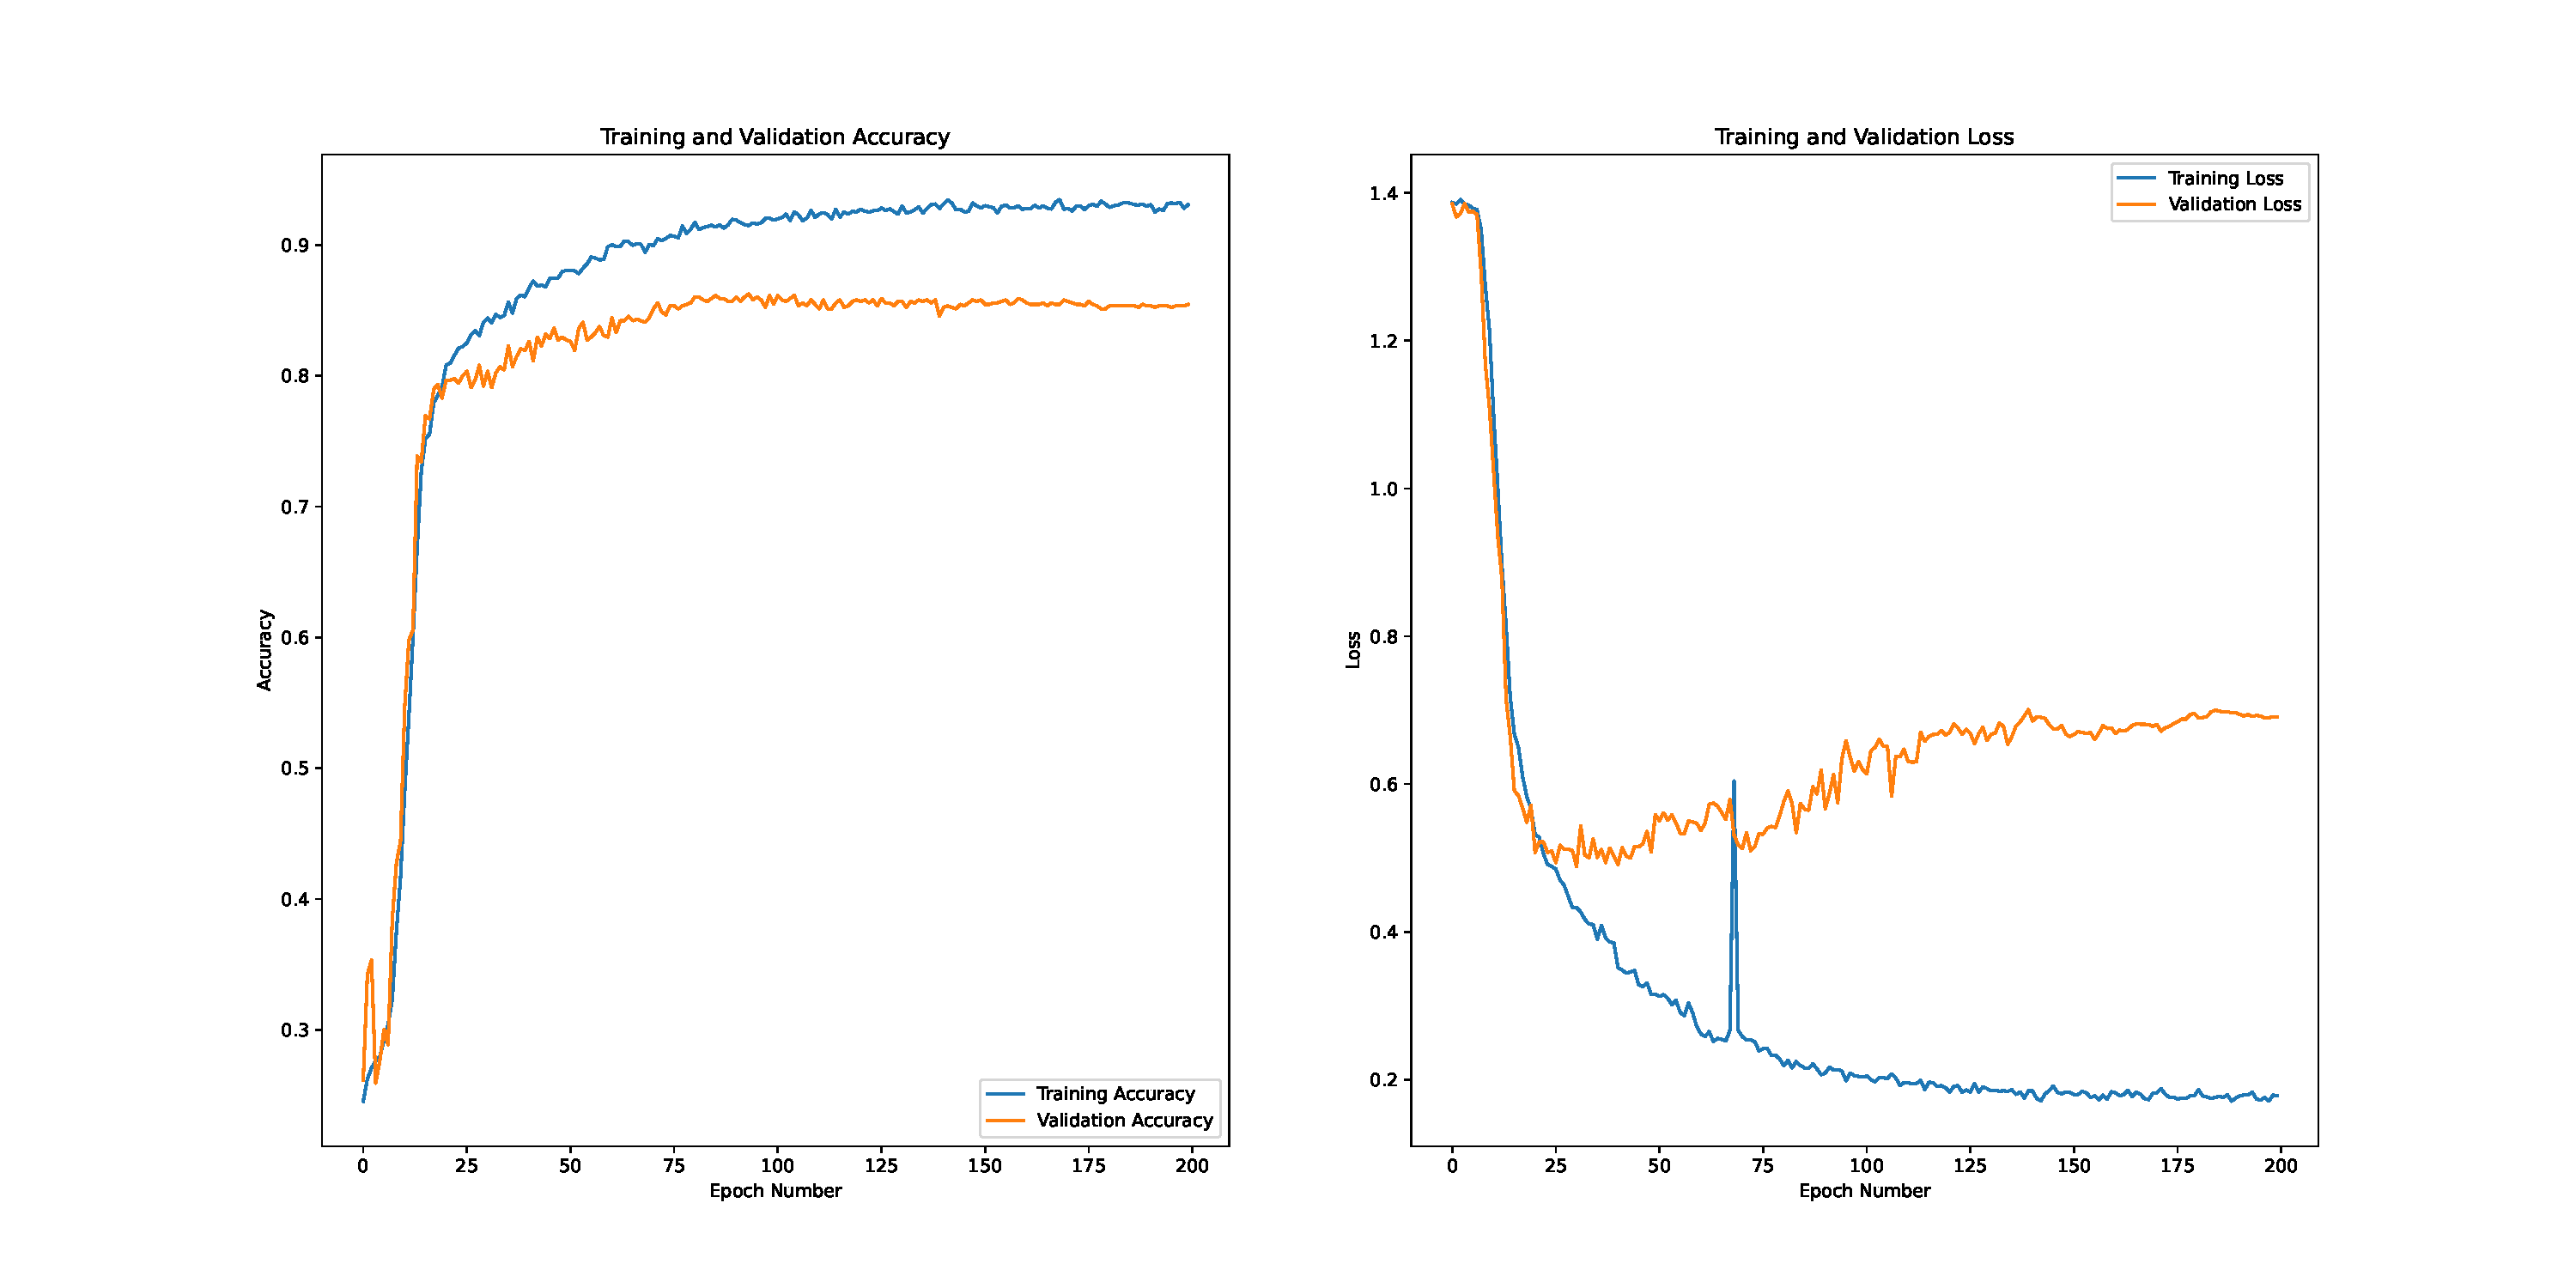
\includegraphics[width=0.5\textwidth]{metrics/5.2 metrics.pdf}}\\
    \subfloat[\centering Experiment 5.3.]{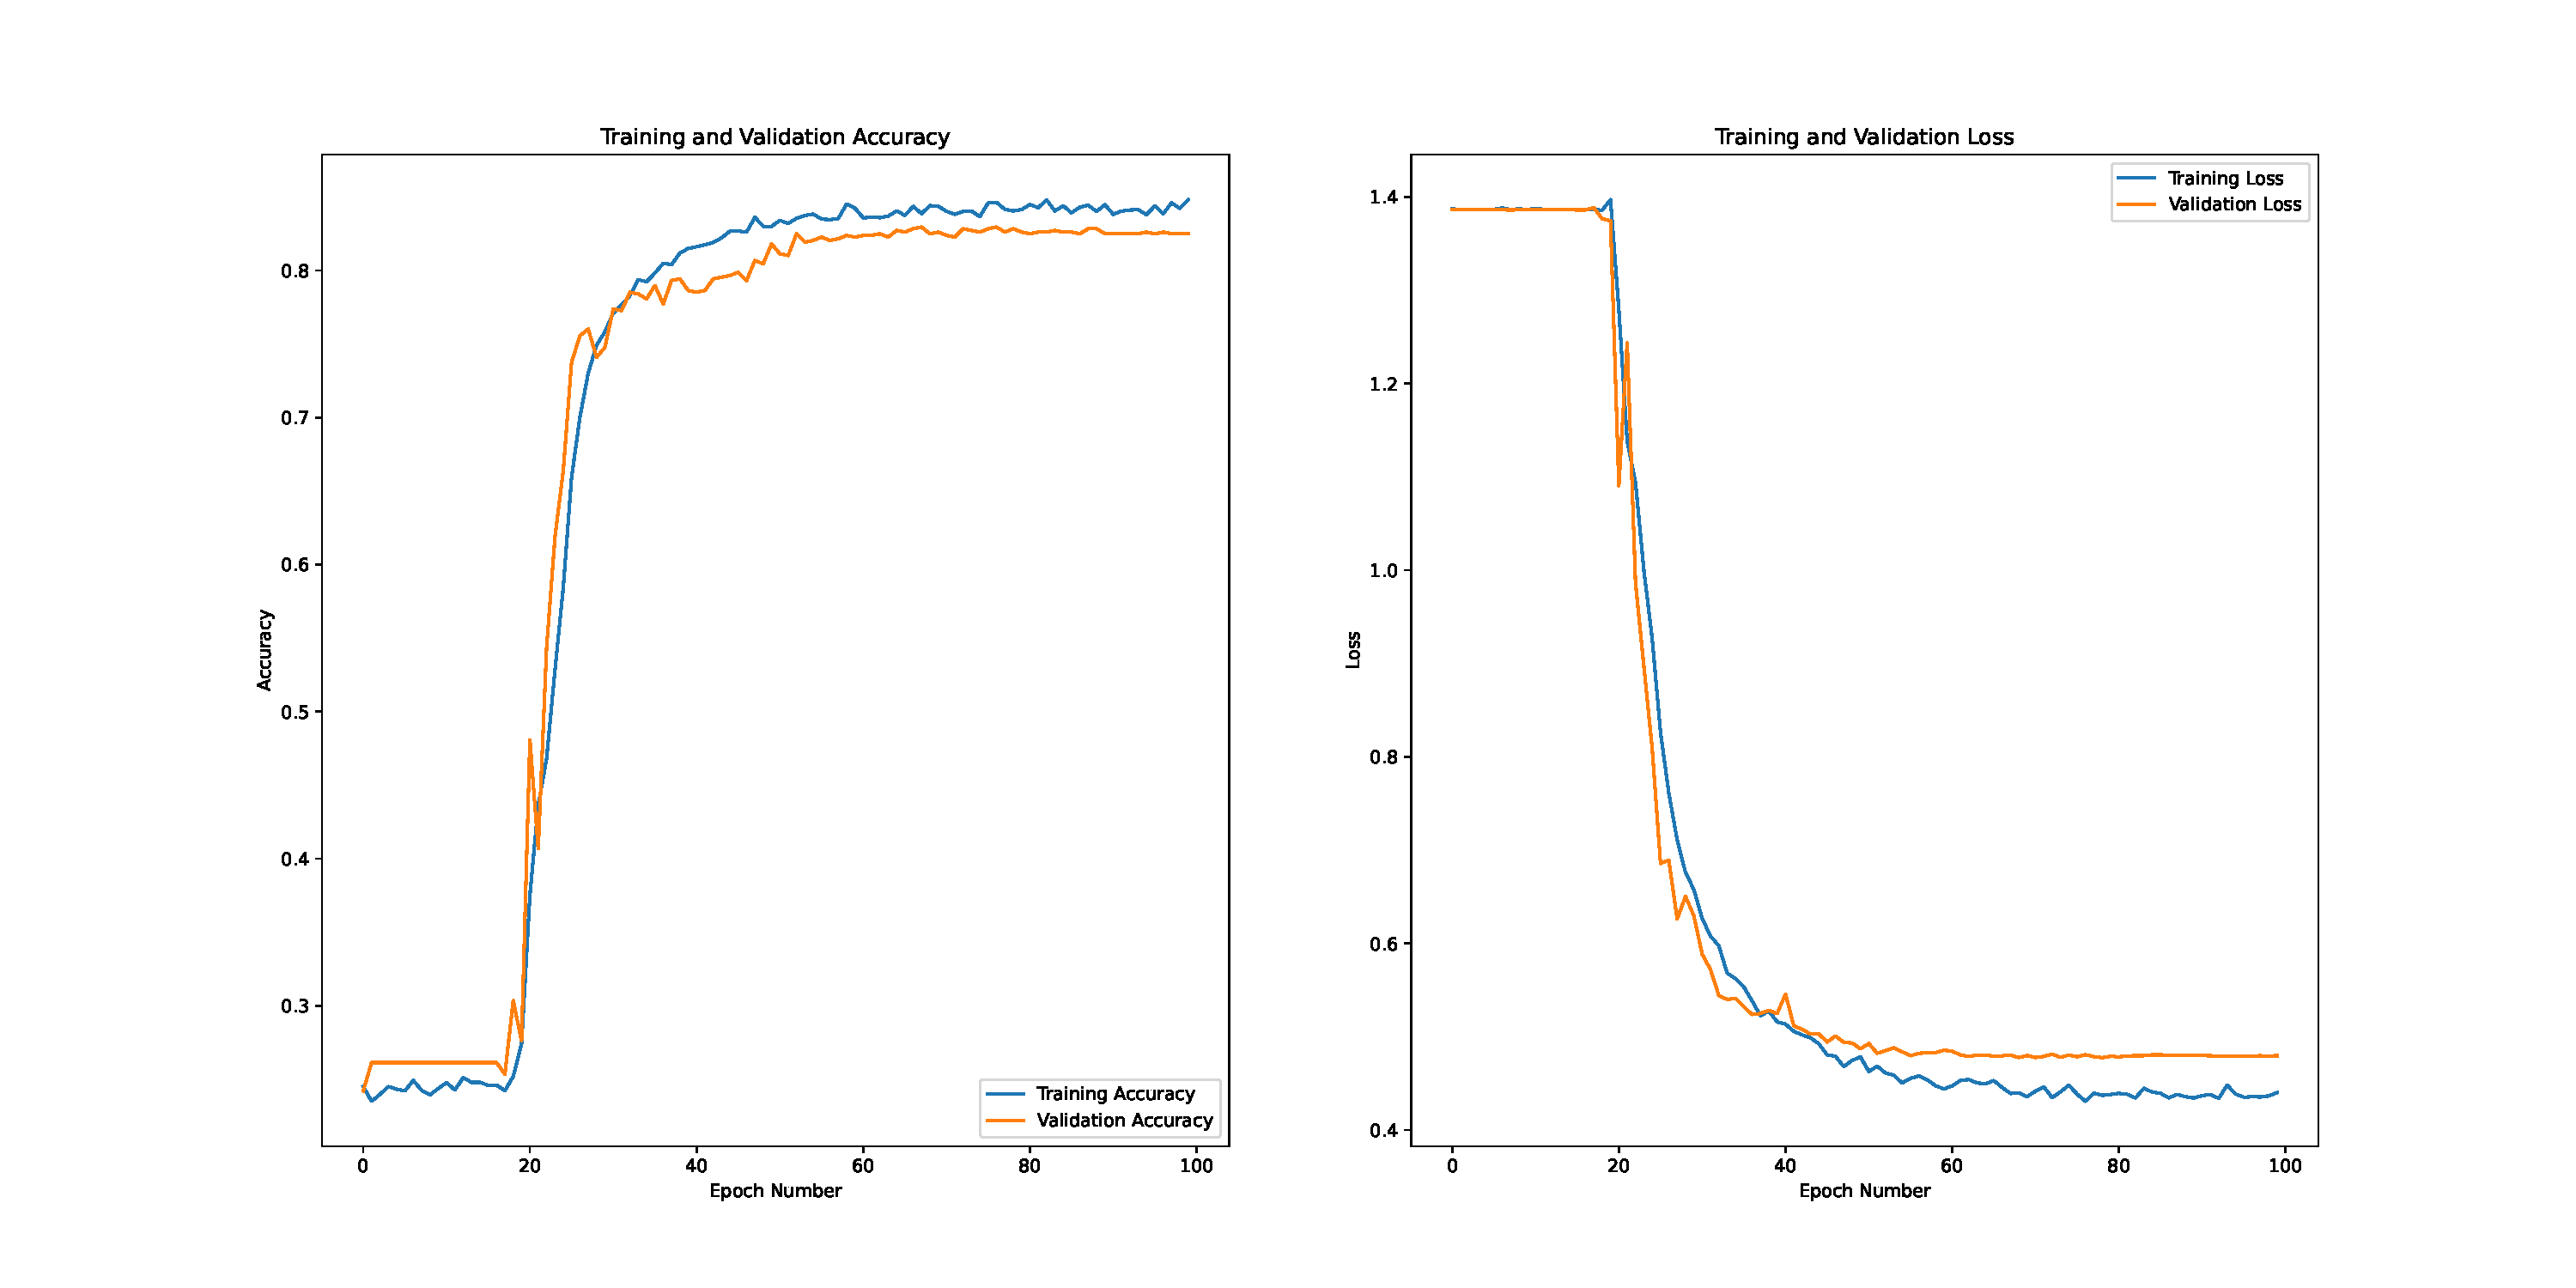
\includegraphics[width=0.5\textwidth]{metrics/5.3 metrics.pdf}}
    \subfloat[\centering Experiment 5.4.]{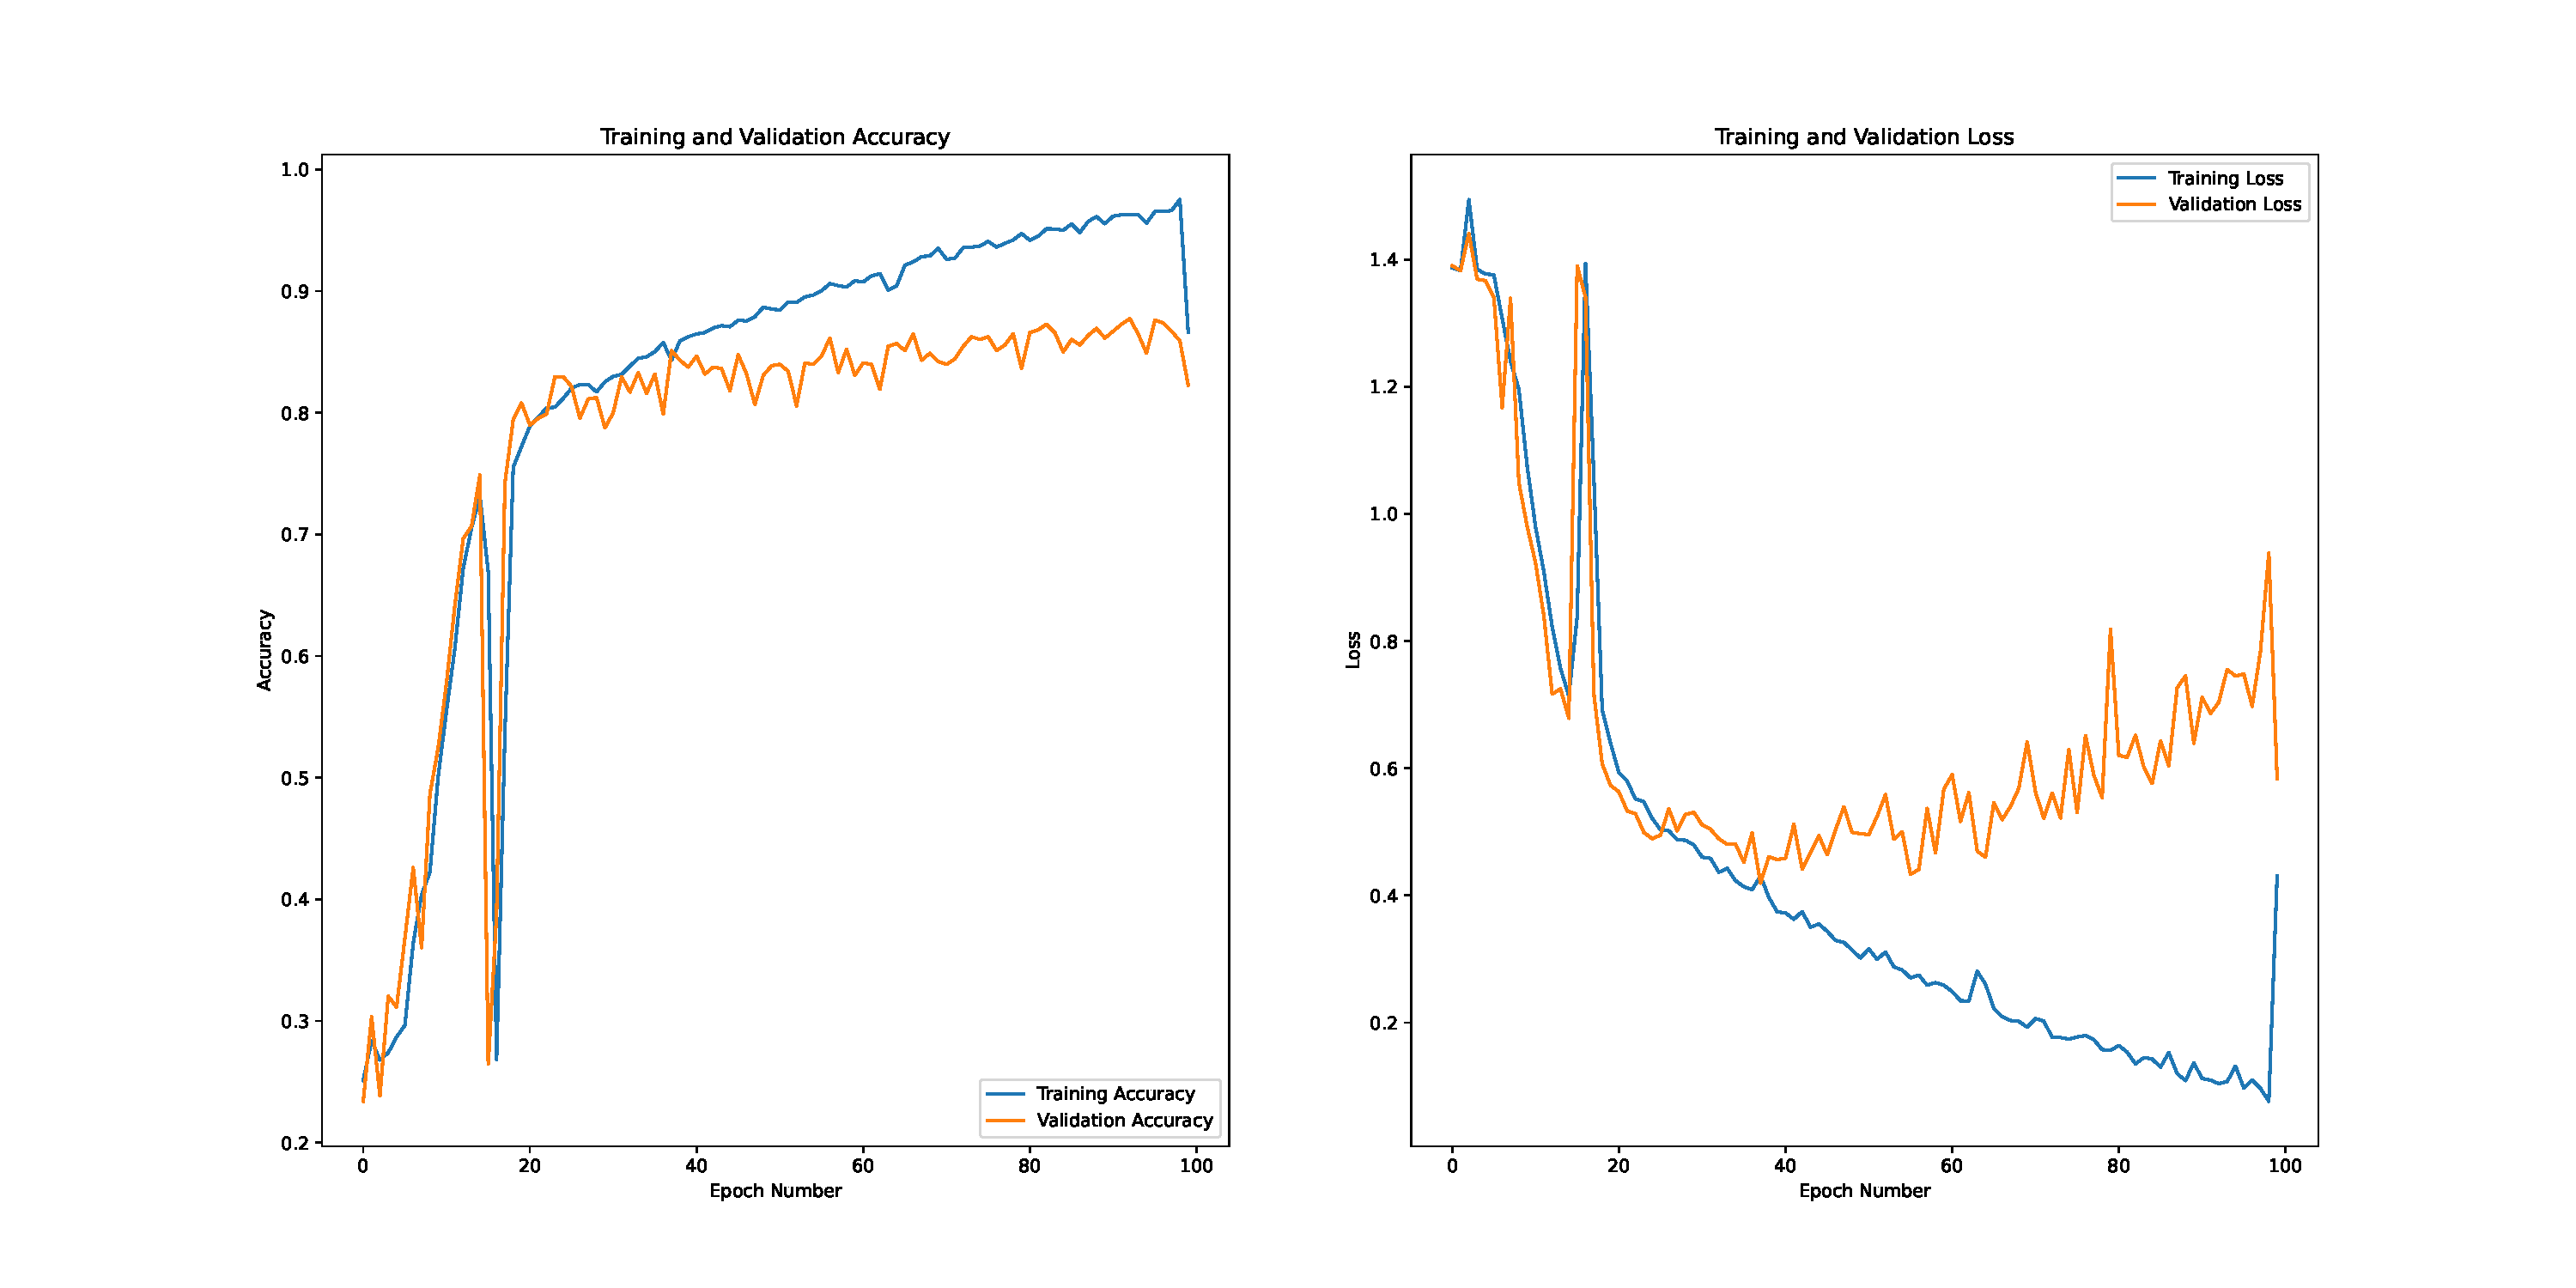
\includegraphics[width=0.5\textwidth]{metrics/5.4 metrics.pdf}}\\
    \subfloat[\centering Experiment 5.5.]{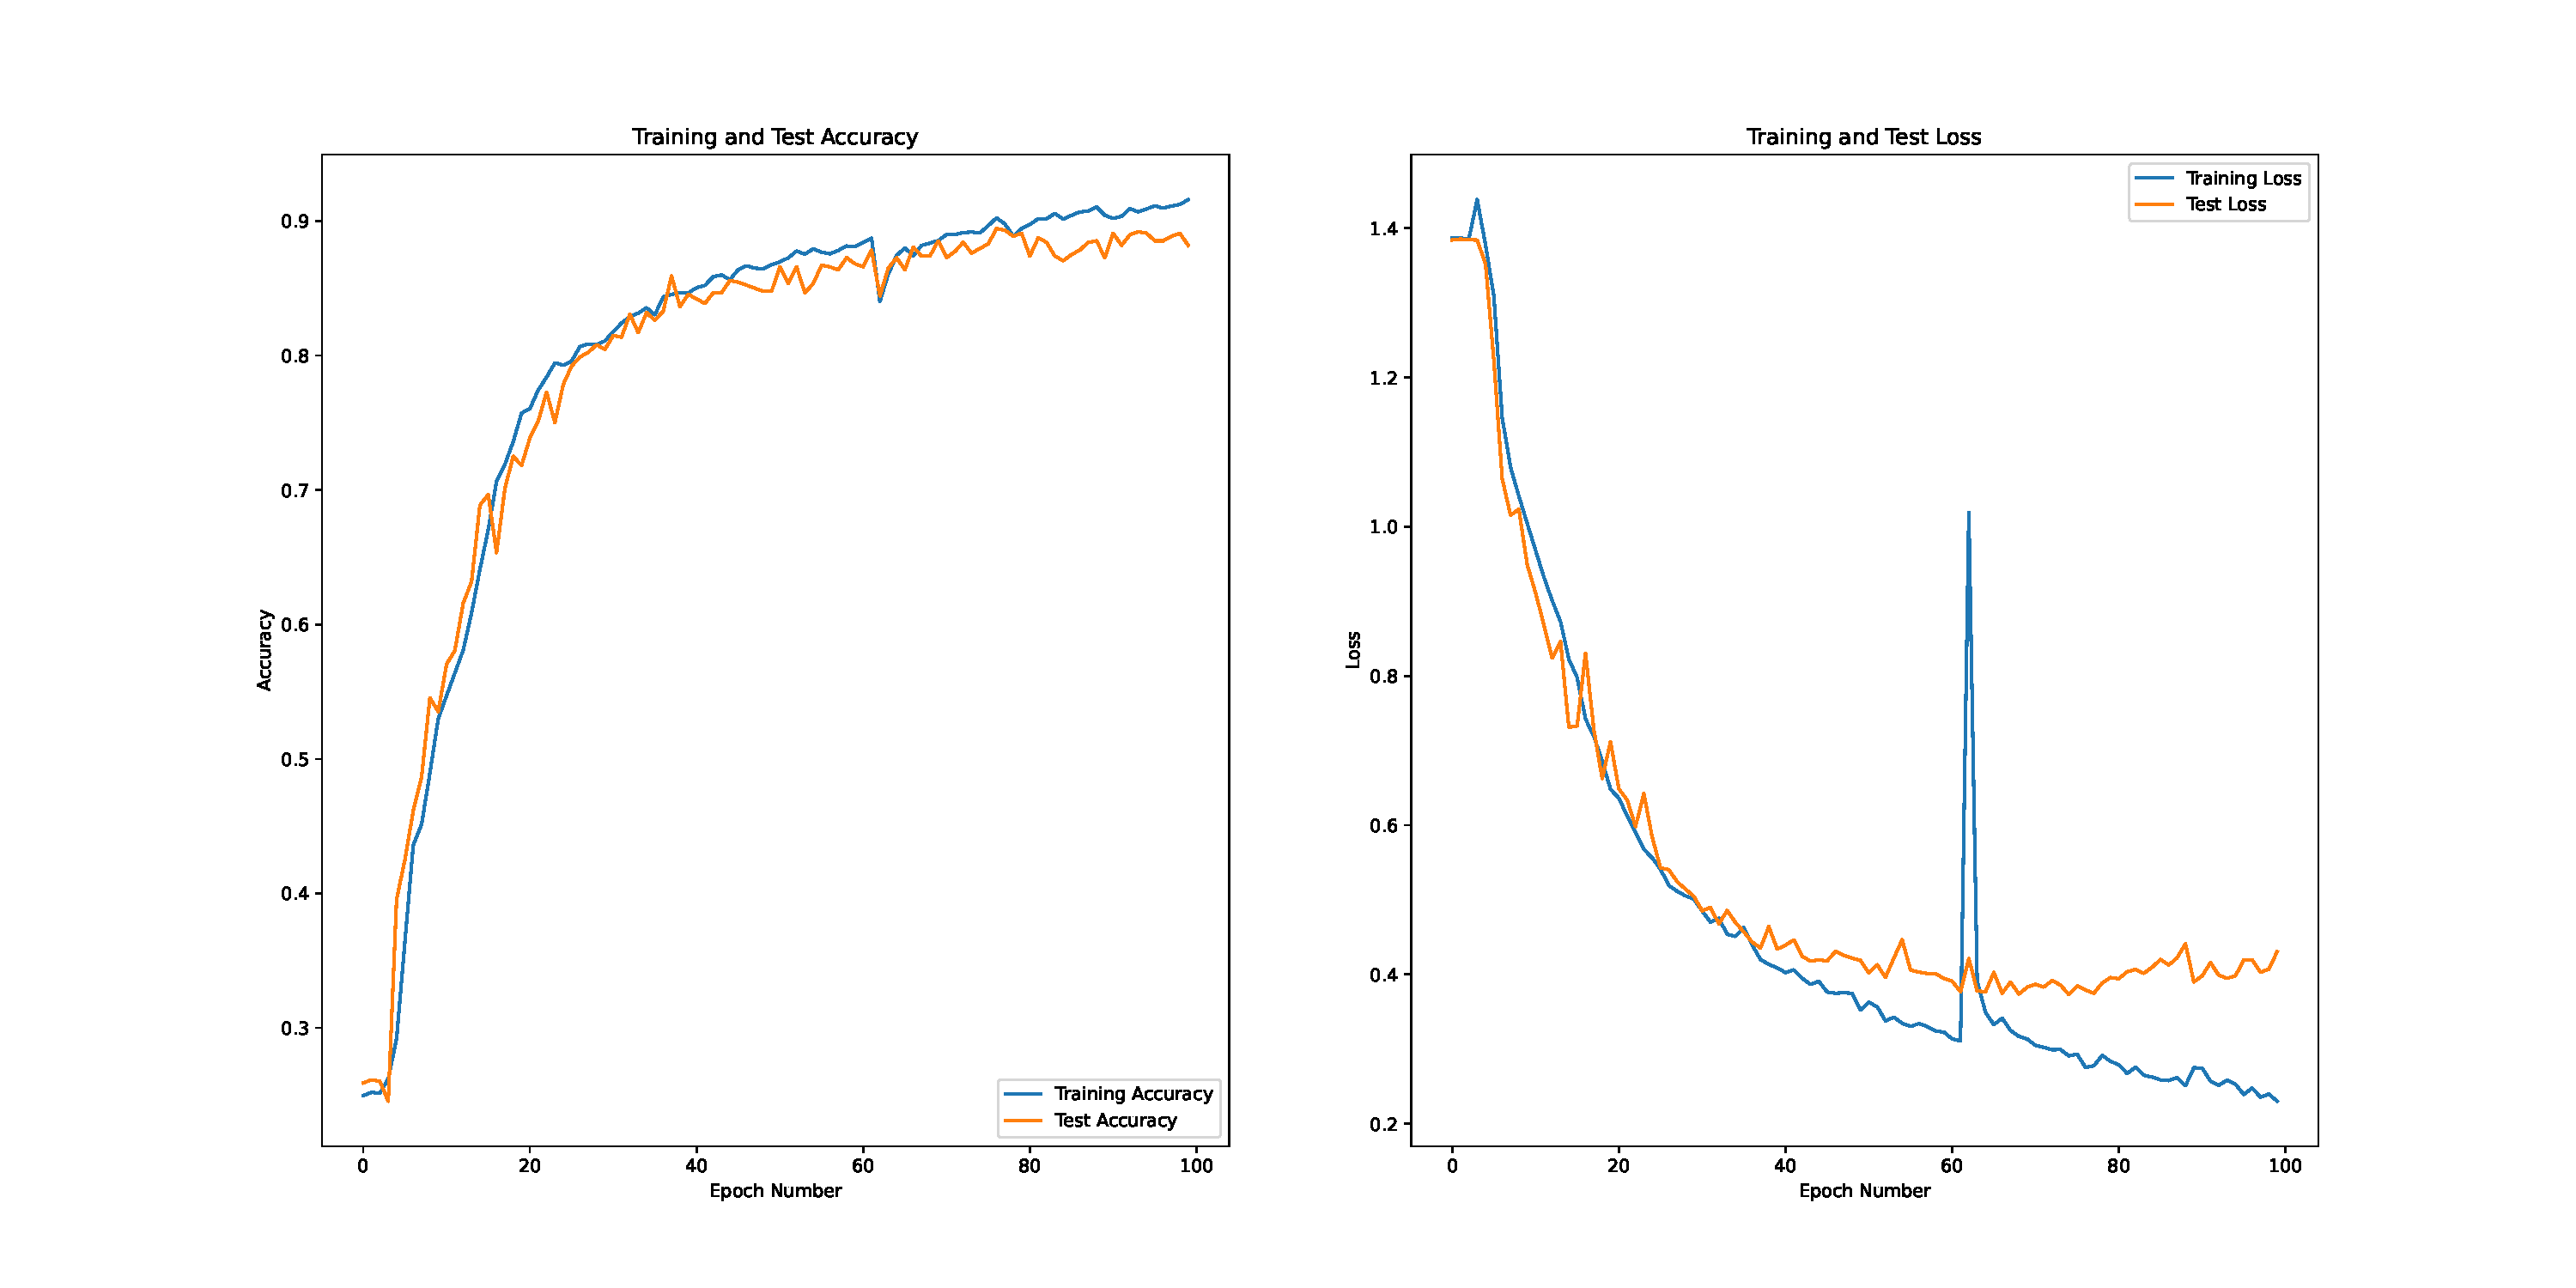
\includegraphics[width=0.5\textwidth]{metrics/5.5 metrics.pdf}}
\caption[Experiment 5 results]{Experiment 5 results. This depicts experiments~5.1, 5.2, 5.3, 5.4 and 5.5. Each of these experiments utilised the same model architecture but varying \acrshort{lr} scheduling methods. 5.1--5.4 utilised manual methods of changing the \acrshort{lr} whilst 5.5 showcased exponential decay.}
\label{fig:5 results}
\end{figure}
\begin{table}
\centering
\begin{tabular}{|c|p{35mm}|c|c|c|} 
 \hline
 Experiment & \acrshort{lr} Configuration & Testing Accuracy & Testing Loss & \acrshort{wer} \\ [0.2ex] 
 \hline
 5.1 & \textbf{Scheduler}: Manual\newline \textbf{Initial \acrshort{lr}}: 0.0001\newline \textbf{Change steps}: 20\newline \textbf{\acrshort{lr} change}: 0.5& \accuracyfiveone & \lossfiveone & \werfiveone \\ 
 \hline
 5.2 & \textbf{Scheduler}: Manual\newline \textbf{Initial \acrshort{lr}}: 0.001\newline \textbf{Change steps}: 20\newline \textbf{\acrshort{lr} change}: 0.5& \accuracyfivetwo & \lossfivetwo & \werfivetwo \\ 
 \hline
 5.3 & \textbf{Scheduler}: Manual\newline \textbf{Initial \acrshort{lr}}: 0.001\newline \textbf{Change steps}: 30\newline \textbf{\acrshort{lr} change}: $e^{-0.1}$& \accuracyfivethree & \lossfivethree & \werfivethree \\ 
 \hline
 5.4 & \textbf{Scheduler}: Manual\newline \textbf{Initial \acrshort{lr}}: 0.001\newline \textbf{Change steps}: 30\newline \textbf{\acrshort{lr} change}: $e^{-0.01}$ & \accuracyfivefour & \lossfivefour & \werfivefour \\ \hline
 5.5 & \textbf{Scheduler}: Exponential decay\newline \textbf{Initial \acrshort{lr}}: 0.001\newline \textbf{Decay steps}: 275\newline \textbf{Decay rate}: 0.9 & \accuracyfivefive & \lossfivefive & \werfivefive \\ 
 \hline
\end{tabular}
\caption[The testing accuracy, loss and \acrshort{wer} for experiment 5]{The testing accuracy, loss and \acrshort{wer} for experiment 5. This shows the settings for each of the different sub-experiments and the resulting testing accuracy and loss.}
\label{table: 5 results}
\end{table}
Although experiment~5.1 did not have improved performance compared with experiment~4.2, the findings from this experiment showed that landmark features are a suitable input for training lip reading models.\\
The reduced performance could be related to the reduced size of the input feature vectors or due to MediaPipe's accuracy. A low probability threshold was utilised during data generation and therefore it could be that the lip landmarks were less accurate than desired. This problem is not present when using visual features, which are just crops of the mouth region.\\
After this finding, different values for the \acrshort{lr} scheduling were assessed to optimise this model further, the results for which are represented within Figure~\ref{fig:5 results} and Table~\ref{table: 5 results}.\\
The next four experiments showed the impact of tuning the scheduler's parameters, significantly altering the performance of the model. When manually altering the \acrshort{lr}, starting with a higher initial \acrshort{lr} and a larger decay rate (leading to smaller changes in the \acrshort{lr}) performed better. Furthermore, Exponential decay performed very well, producing one of the best models in this research yet.\\
The \acrshort{lr} setting presented in experiment~5.4 performed the best. However, the \acrshort{lr} scheduler from experiment~5.5 was taken forwards. Although this model had worse testing metrics, the spiking within the accuracy and loss was far decreased compared with the other methods. Additionally, \gls{overfitting} appeared to have been diminished. This reliability is more useful than hyperparameters configured for a specific experiment. Experiment~5.5's \acrshort{lr} scheduling is more general and thus will be carried forward, rather than the settings for experiment~5.5.
\section{Experiment 6: Data Augmentation}
\label{sec: Experiment 6}
% Experiment 11
% More \gls{data_augmentation} 
\subsection{Model Architecture}
In Section~\ref{sec: Experiment 5}, although \gls{overfitting} was reduced, there was still divergence among the loss and accuracy in the later epochs. Thus, further methods of \gls{data_augmentation} were assessed to reduce this effect.\\
The method of \gls{data_augmentation} that was employed was a set of random rotations. Each of the data samples were randomly rotated and the new samples were added again to the dataset, to bolster the amount of training data. The same rotation was applied to each lip landmark within a frame, and each frame of a given video. The rotations were in the range $[-\frac{\pi}{8}, -0.1]$ and $[0.1, \frac{\pi}{8}]$. This was to ensure that the generated samples were not too similar to the originals. Normally, viewers will be upright and not rotated, so rotations were kept minimal.\\
Otherwise, the architecture for this experiment was identical to experiment~5.5.
\subsection{Results and Evaluation}
\begin{figure}
\centering
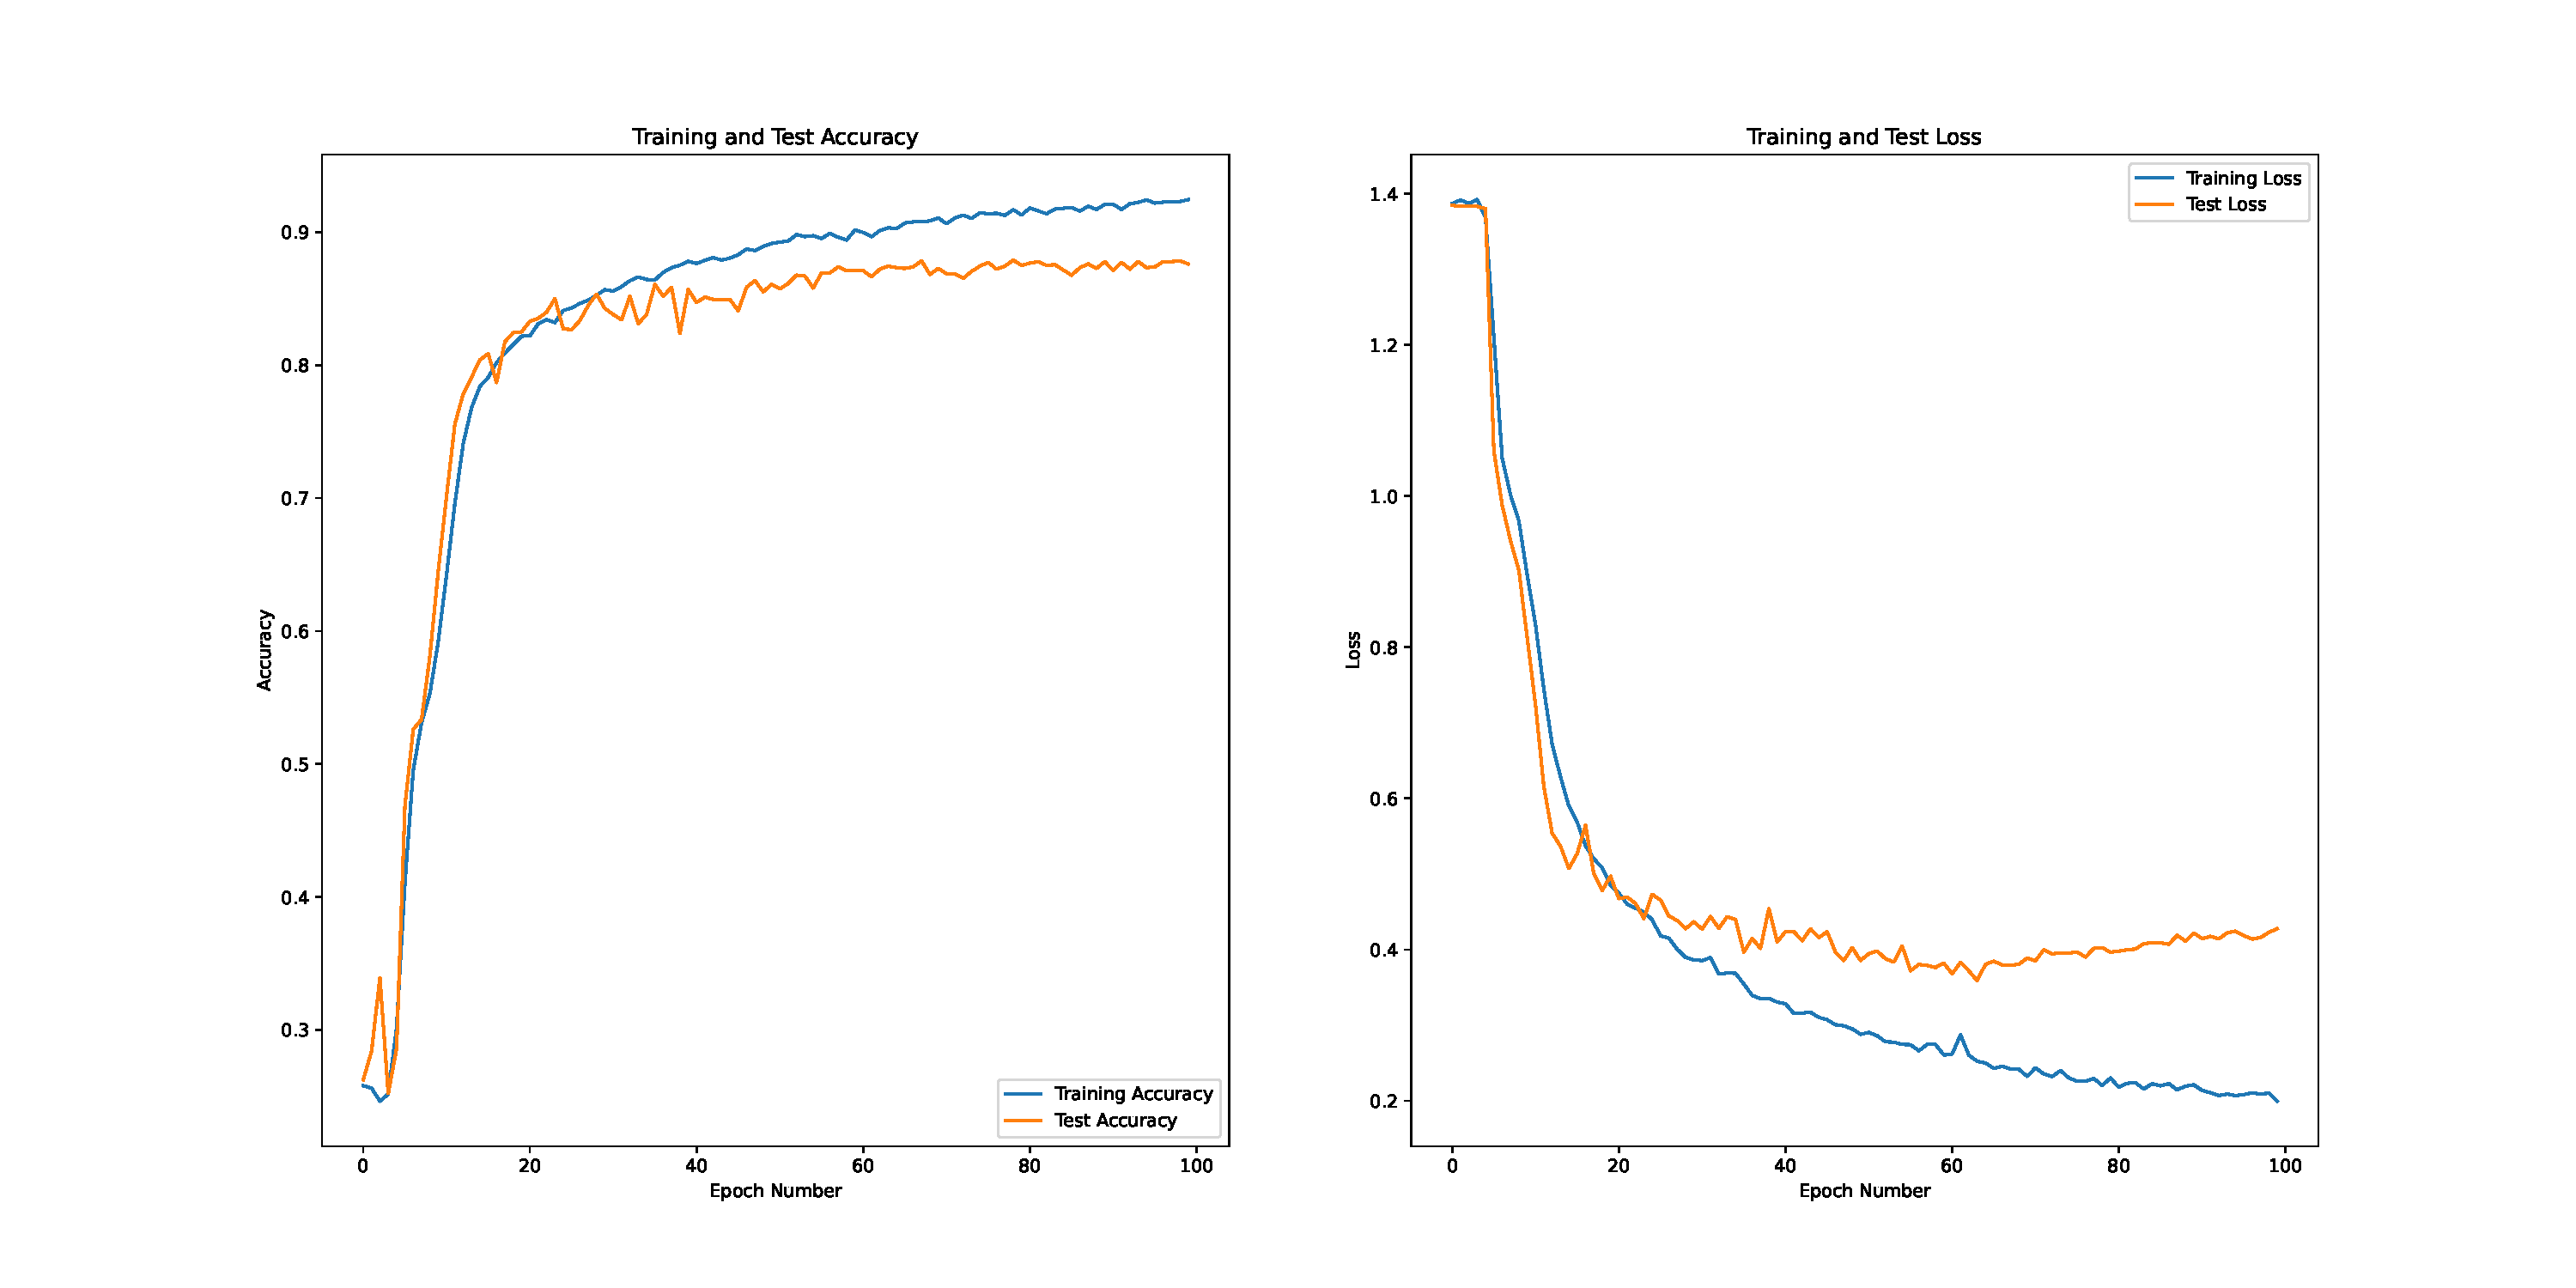
\includegraphics[width=1\textwidth]{metrics/6 metrics.pdf}
\caption[Experiment 6 results]{Experiment 6 results. This shows the impact of a further set of \gls{data_augmentation}s: landmark rotations. The result of this shows decreased performance and a more overfit model.}
\label{fig:6 results}
\end{figure}
\begin{table}
\centering
\begin{tabular}{|c|c|c|c|} 
 \hline
 Experiment &  Testing Accuracy & Testing Loss & \acrshort{wer} \\ [0.2ex] 
 \hline
 6 & \accuracysix & \losssix & \wersix \\ 
 \hline
\end{tabular}
\caption[The testing accuracy, loss and \acrshort{wer} for experiment 6]{The testing accuracy, loss and \acrshort{wer} for experiment 6.}
\label{table: 6 results}
\end{table}
Shown in Figure~\ref{fig:6 results} and Table~\ref{table: 6 results}, the results of this experiment reflected reduced performance, showing that the \gls{data_augmentation} was not beneficial. This may be due to the random rotations not being drastic enough or the amount of \gls{data_augmentation} being too much.\\
Previous to this experiment, each data sample was technically in the dataset twice already: having been augmented once. Random rotations meant that single data samples, although augmented, were presented to the model up to four times. Consequently, \gls{overfitting} could have been due to the structure of the sentences within the data samples, and repeated samples with these structures. Repeated noise might have been causing \gls{overfitting}. Consequently, this extra \gls{data_augmentation} method was not applied to further experiments.
\section{Experiment 7: Transformer Architecture}
\label{sec: Experiment 7}
% Experiment 12a
% Attention/transformer 
\subsection{Model Architecture}
\begin{figure}
\centering
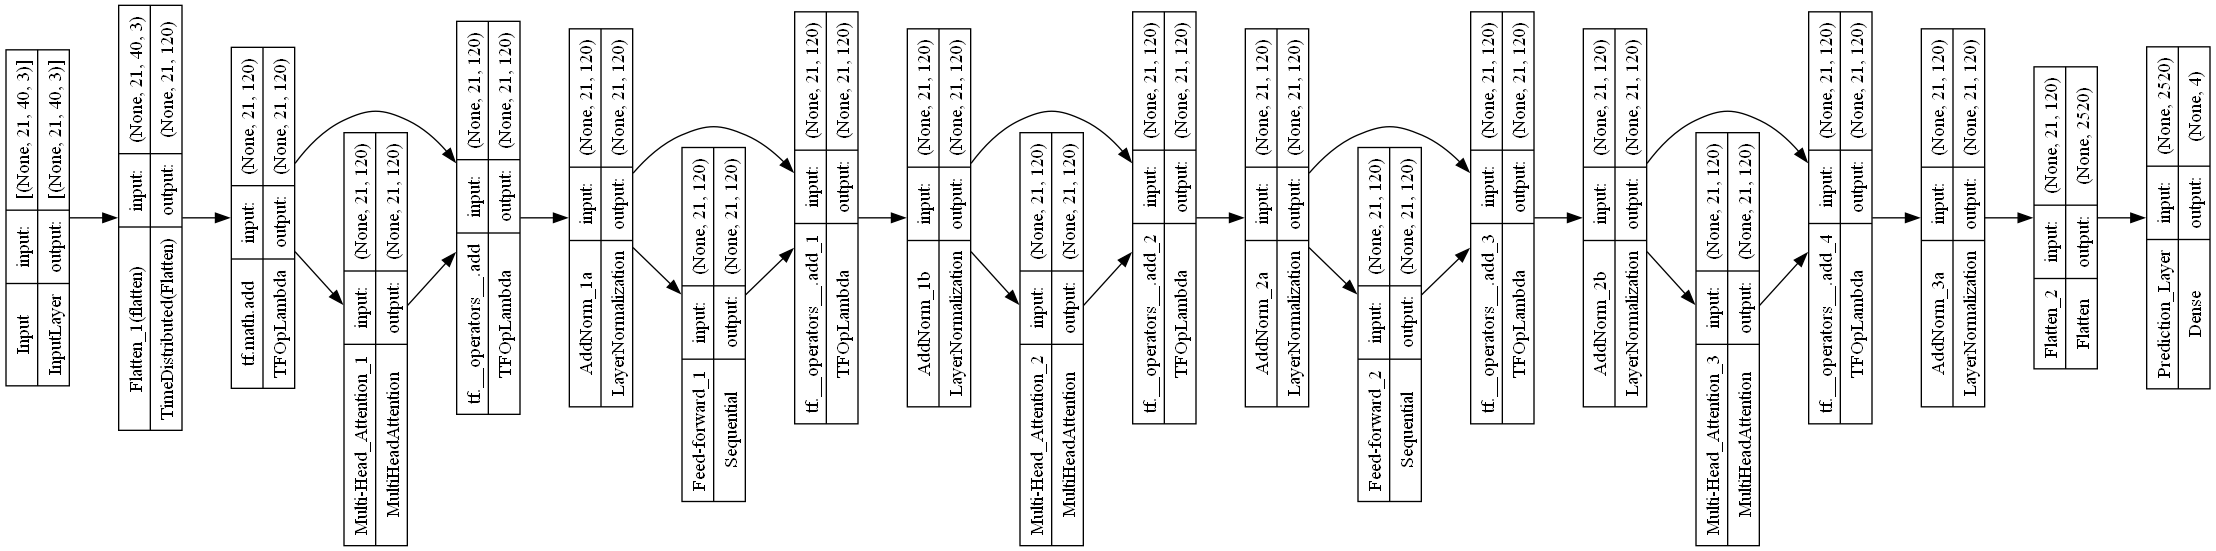
\includegraphics[width=0.9\textwidth]{model architectures/7 architecture.png}
\caption[Experiment 7 architecture]{Experiment 7 architecture. This comprised of an input layer accepting landmark features followed by a series of three encoder blocks. Encoder blocks were made up of multi-head attention blocks and \emph{Add\&Norm} layers. Finally, a feed-forward network was used at the end, before the final hidden representation was fed into a prediction layer.}
\label{fig:7 architecture}
\end{figure}
For this experiment a different model architecture was used, shown in Figure~\ref{fig:7 architecture}. The mechanism of attention, explained in Section~\ref{sec: Attention}, was employed to construct an encoder \gls{transformer} architecture.\\
Landmark features were input and combined with a positional encoding layer\footnote{\url{https://keras.io/api/layers/core_layers/embedding/}}. The output of this was fed into a series of encoder blocks, made up of multi-head attention\footnote{\url{https://keras.io/api/layers/attention_layers/multi_head_attention/}} and \emph{Add\&Norm} layers\footnote{\url{https://keras.io/api/layers/normalization_layers/layer_normalization/}}. The output from this was then fed into a simple feed-forward network and then a dense layer for classification. The purpose of this experiment was to investigate the potential benefits of attention and a \gls{transformer} architecture for lip reading.\\
The same \acrshort{lr} scheduling and batch size was used as experiment 5.5.
\subsection{Results and Evaluation}
\begin{figure}
\centering
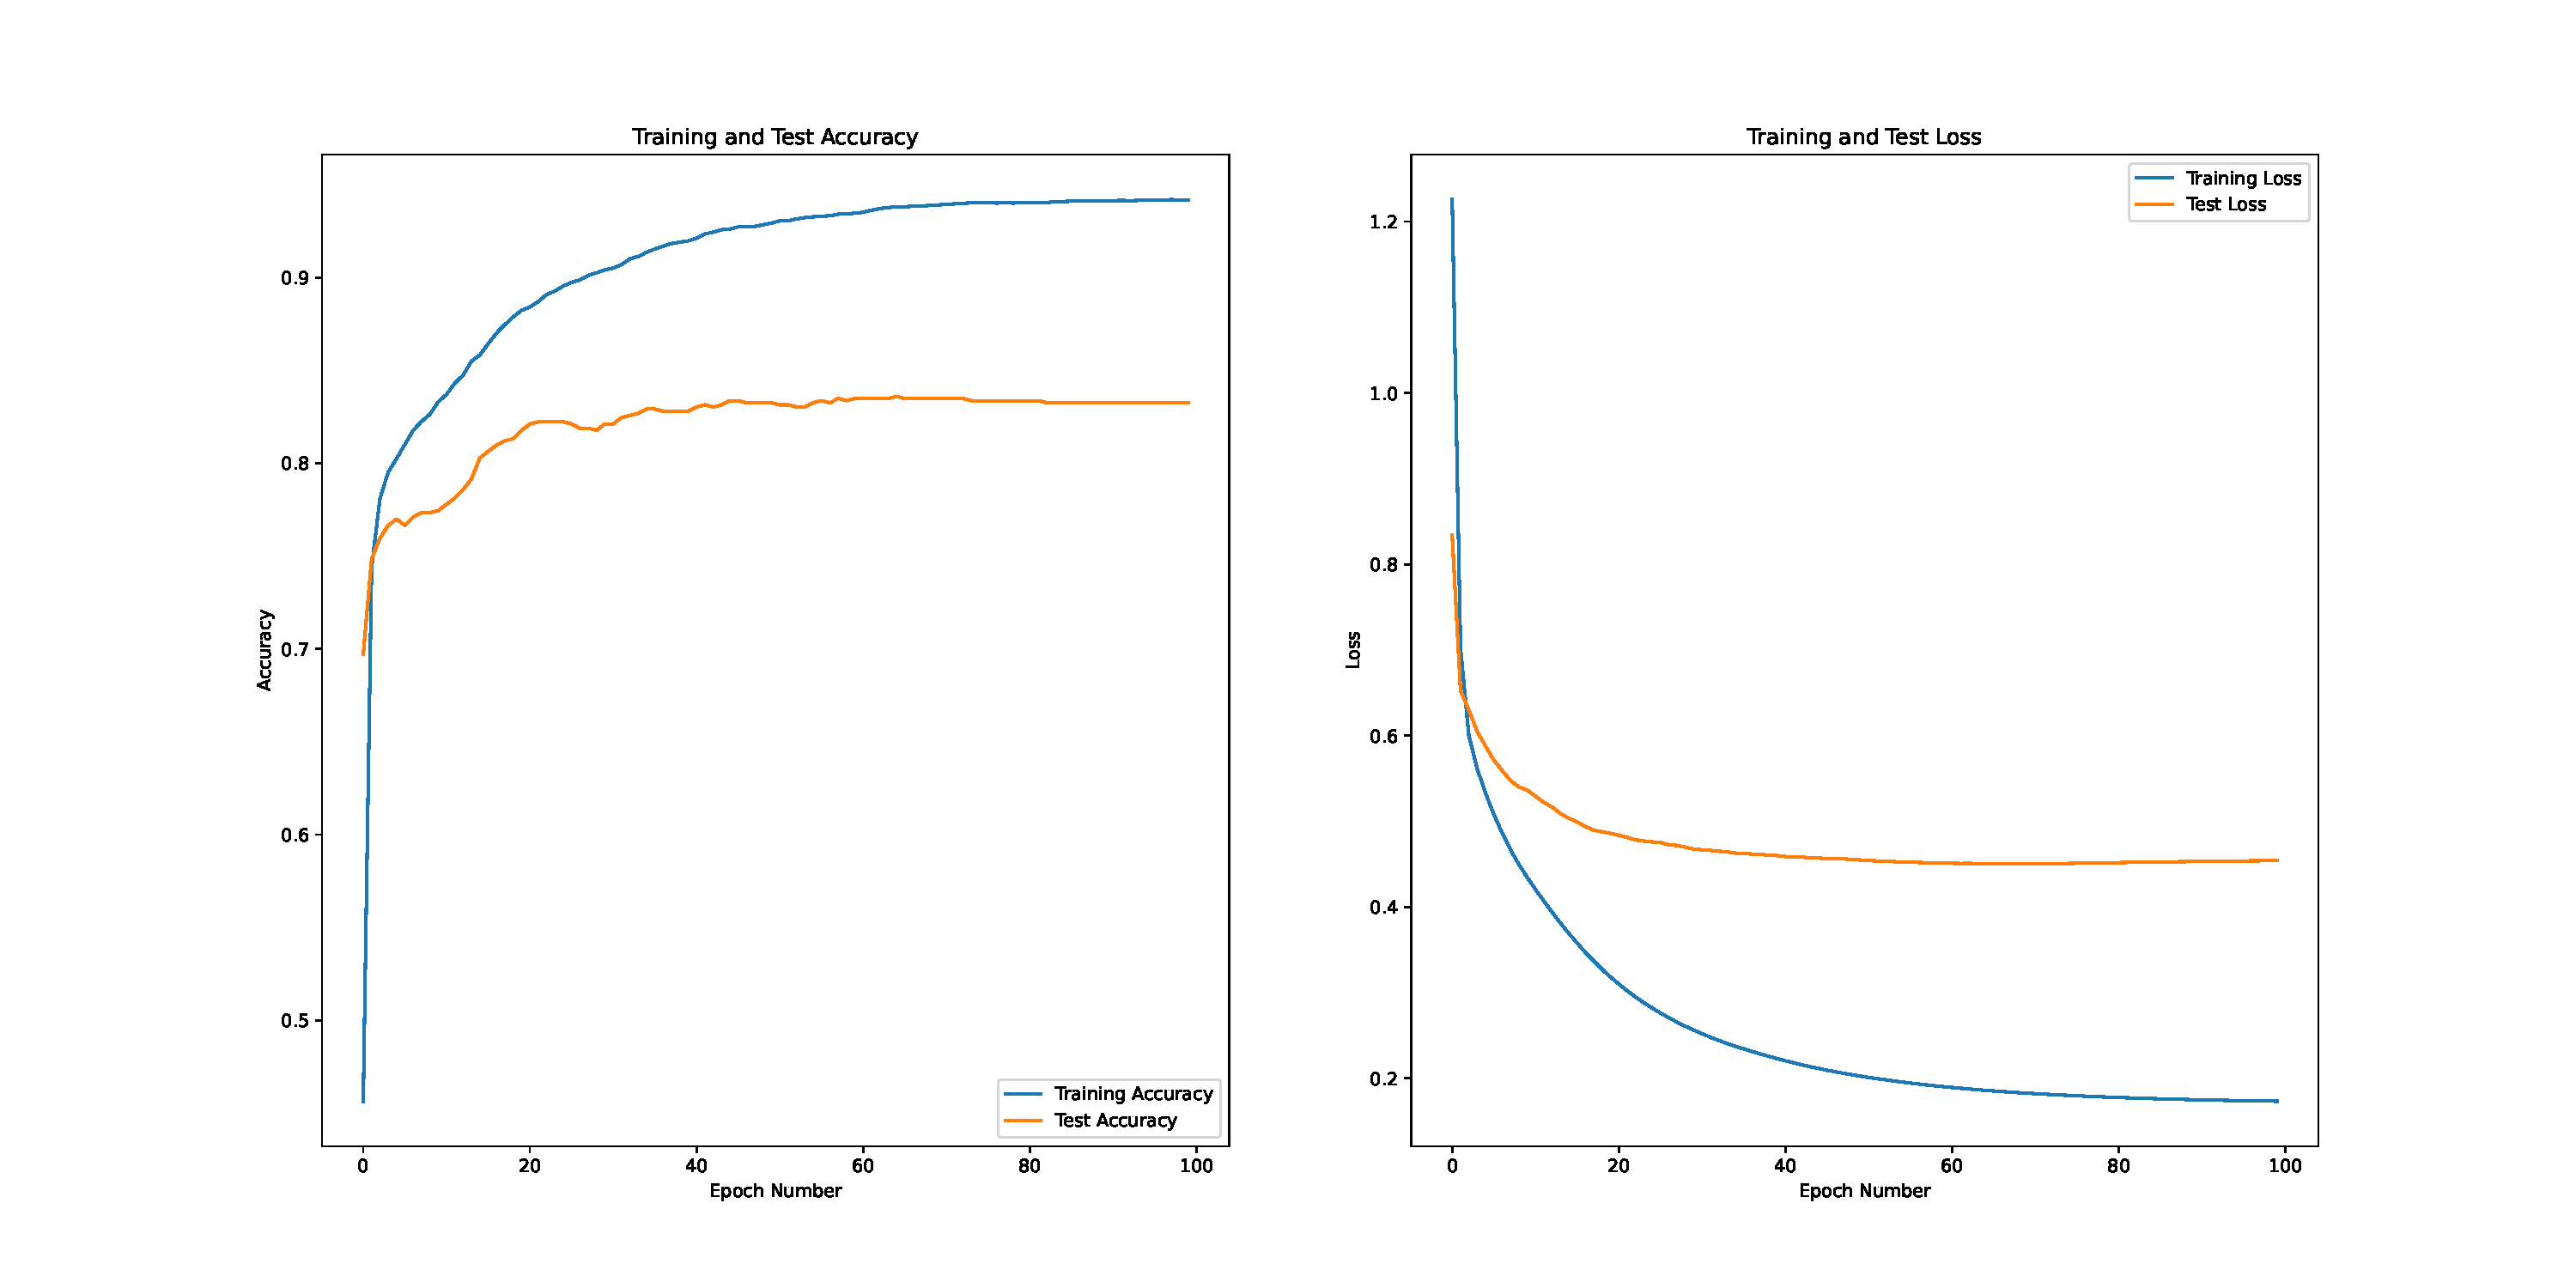
\includegraphics[width=1\textwidth]{metrics/7 metrics.pdf}
\caption{Experiment 7 results}
\label{fig:7 results}
\end{figure}
\begin{table}
\centering
\begin{tabular}{|c|c|c|c|} 
 \hline
 Experiment &  Testing Accuracy & Testing Loss & \acrshort{wer} \\ [0.2ex] 
 \hline
 7 & \accuracyseven & \lossseven & \werseven \\ % Original transformer architecture
 \hline
\end{tabular}
\caption{The testing accuracy, loss and \acrshort{wer} for experiment 7.}
\label{table: 7 results}
\end{table}
Shown in Figure~\ref{fig:7 results} and Table~\ref{table: 7 results}, the resulting model performed worse than previous models. \Gls{overfitting} occurred but, as a proof of concept, the \gls{transformer} architecture for lip reading was highly successful. Therefore, further experimentation was carried out to assess this architecture further.
\section{Experiment 8: Image and Landmarks}
\label{sec: Experiment 8}
% Experiment 12c
% Image & landmark data combined
\subsection{Model Architecture}
\begin{figure}
\centering
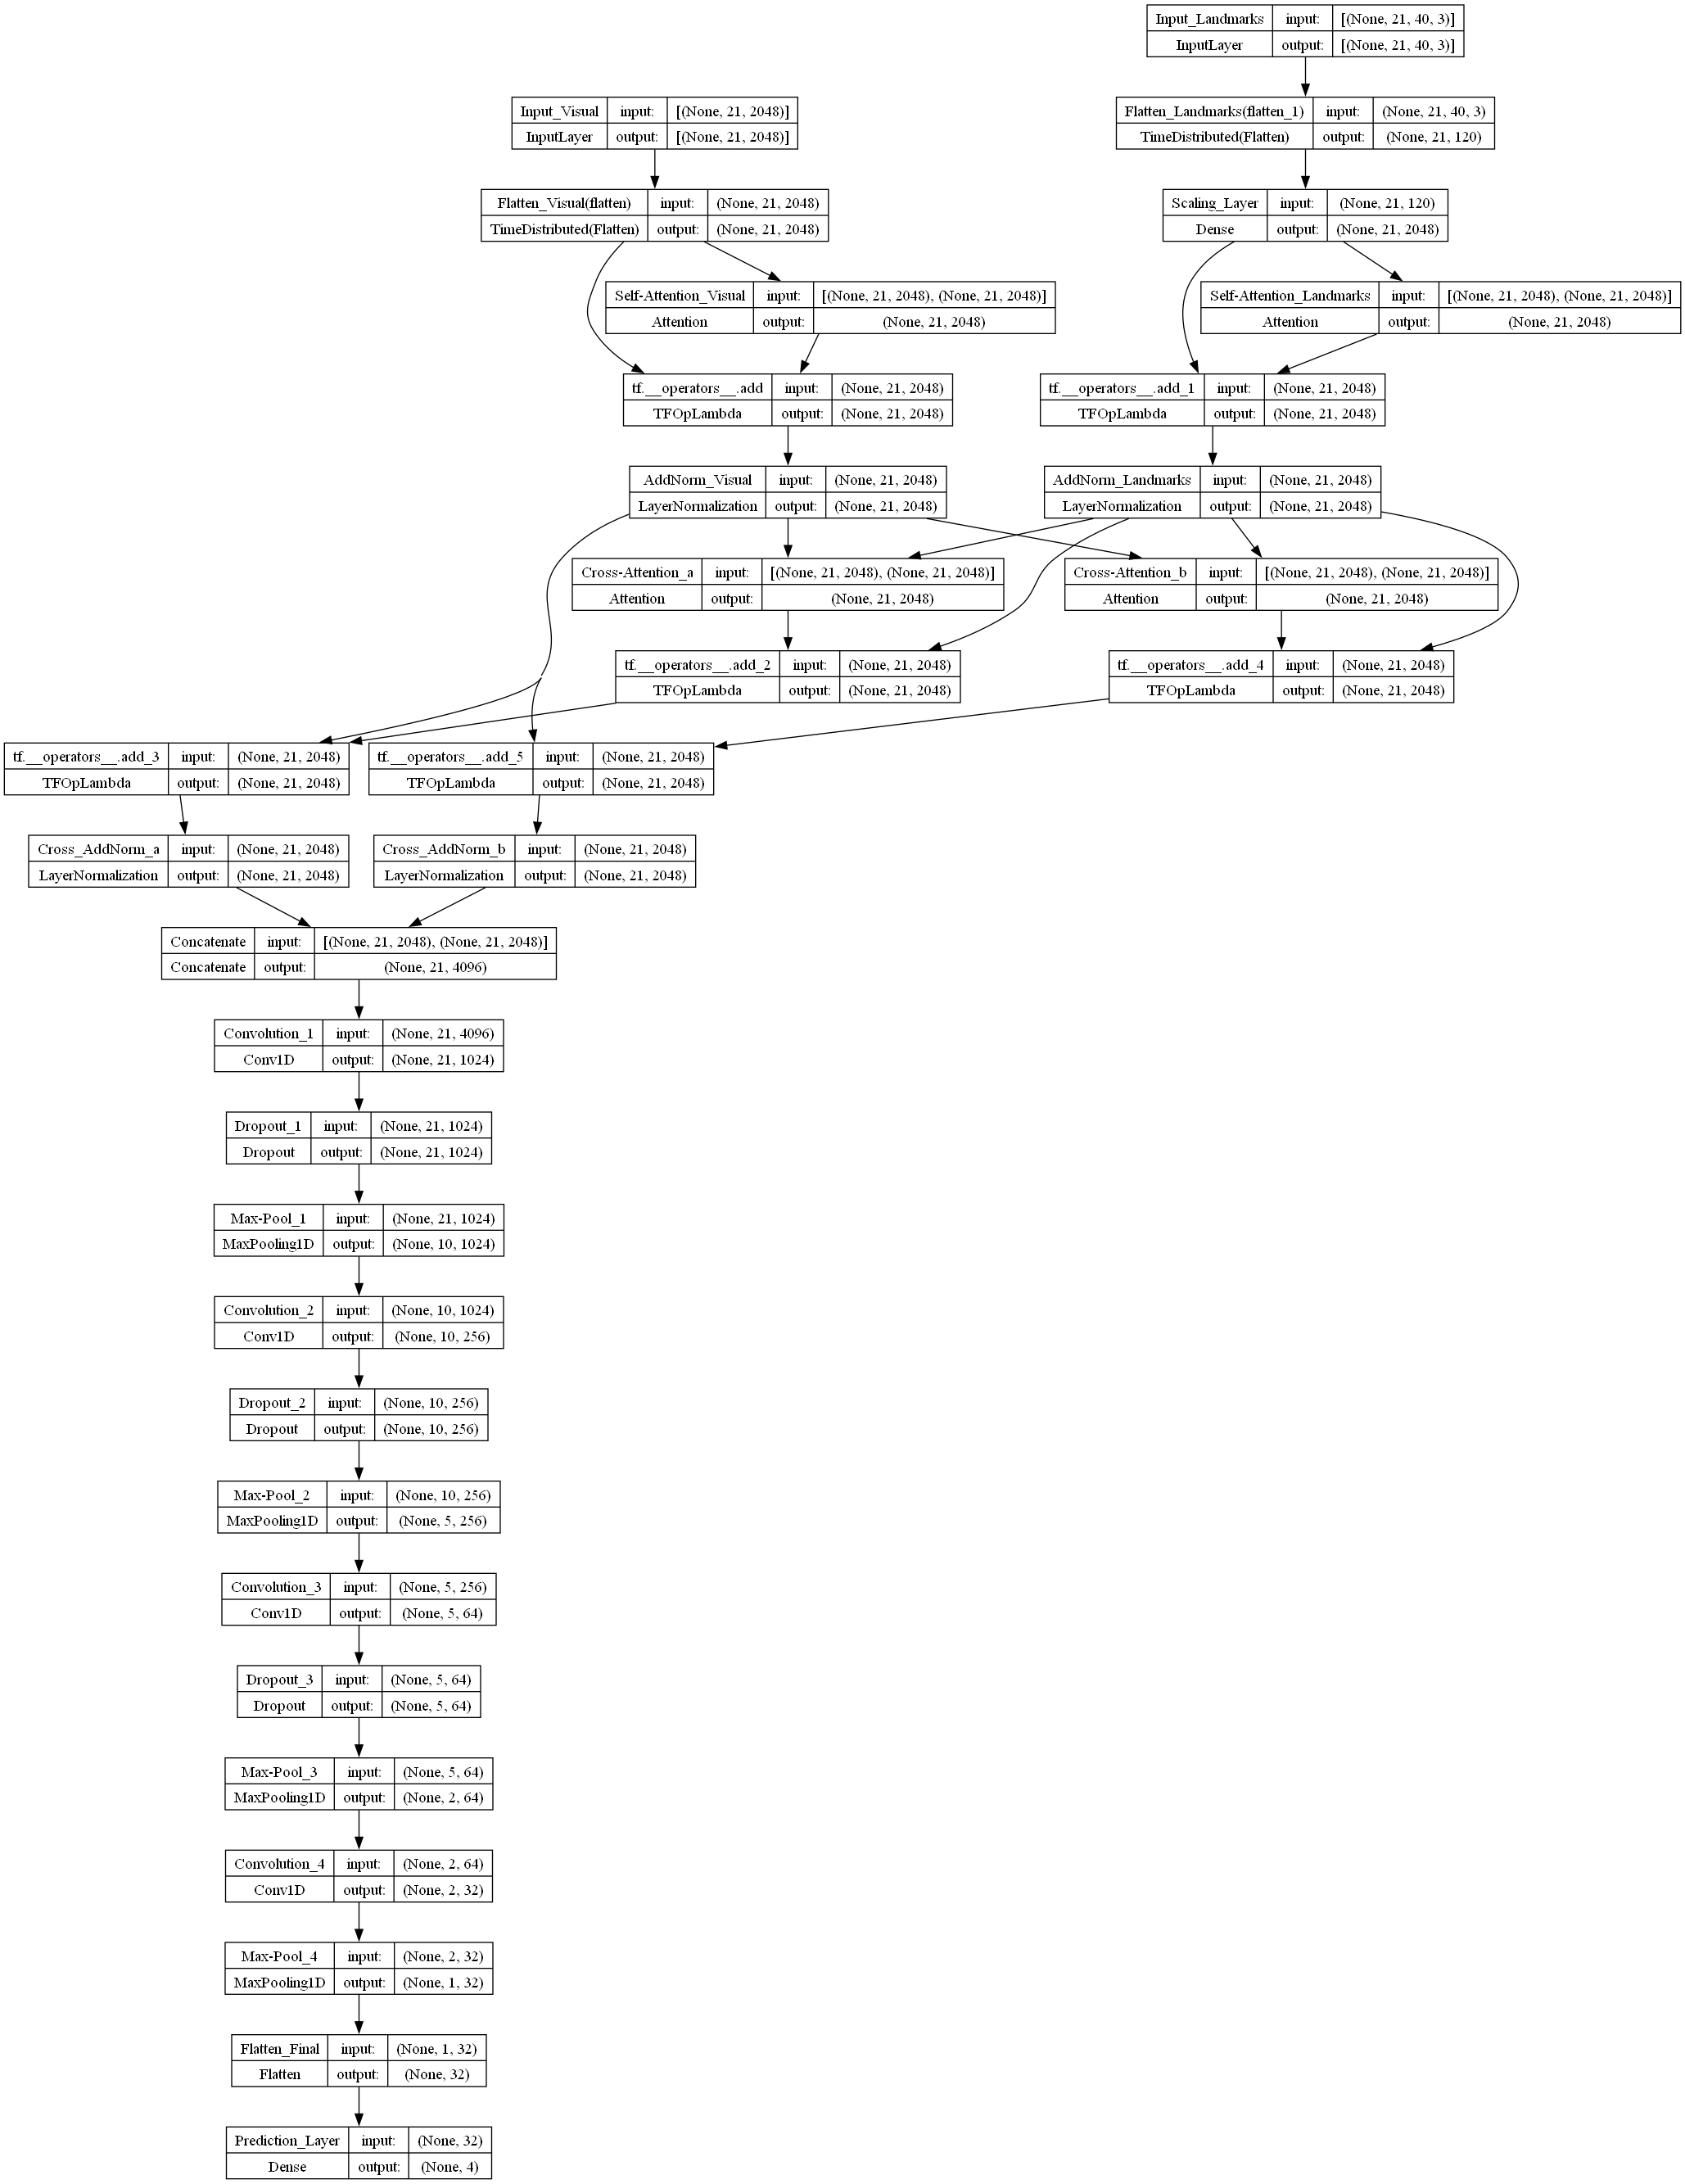
\includegraphics[width=1\textwidth]{model architectures/8 architecture.png}
\caption[Experiment 8 architecture]{Experiment 8 architecture. This architecture was based on the work of Xue et al.~\cite{lipreading_with_attention}. The model took both visual and landmark features as input to an encoder. The encoder employed self-attention and \emph{Add\&Norm} on either input before using cross-attention between them. The output was then fed into a series of convolutional layers and the prediction layer.}
\label{fig:8 architecture}
\end{figure}
For this experiment, the \gls{transformer} architecture was adapted to improve performance. Inspired by Xue et al.~\cite{lipreading_with_attention}, both visual and landmark features were utilised as inputs to a model, to investigate their potential combined benefit.\\ 
As depicted within Figure~\ref{fig:8 architecture}, visual and landmark features were fed into independent self-attention blocks. These blocks consisted of dot-product self-attention\footnote{\url{https://keras.io/api/layers/attention_layers/attention/}} and \emph{Add\&Norm} layers\footnote{\url{https://keras.io/api/layers/normalization_layers/layer_normalization/}}. The two streams were then fed into similar cross-attention blocks. These blocks instead used the query from one input stream and the key from the alternate stream, hence comparing the two streams and, therefore, formulating cross-attention. The output from this was passed through a further \emph{Add\&Norm} layer before being input into a \acrshort{cnn}. Xue et al. utilised a series of \acrshort{gru} units but our research found that convolutional layers performed better.\\
The same \acrshort{lr} scheduler was used as in experiment 5.5 for better comparison of the new model architecture.
\subsection{Results and Evaluation}
\begin{figure}
\centering
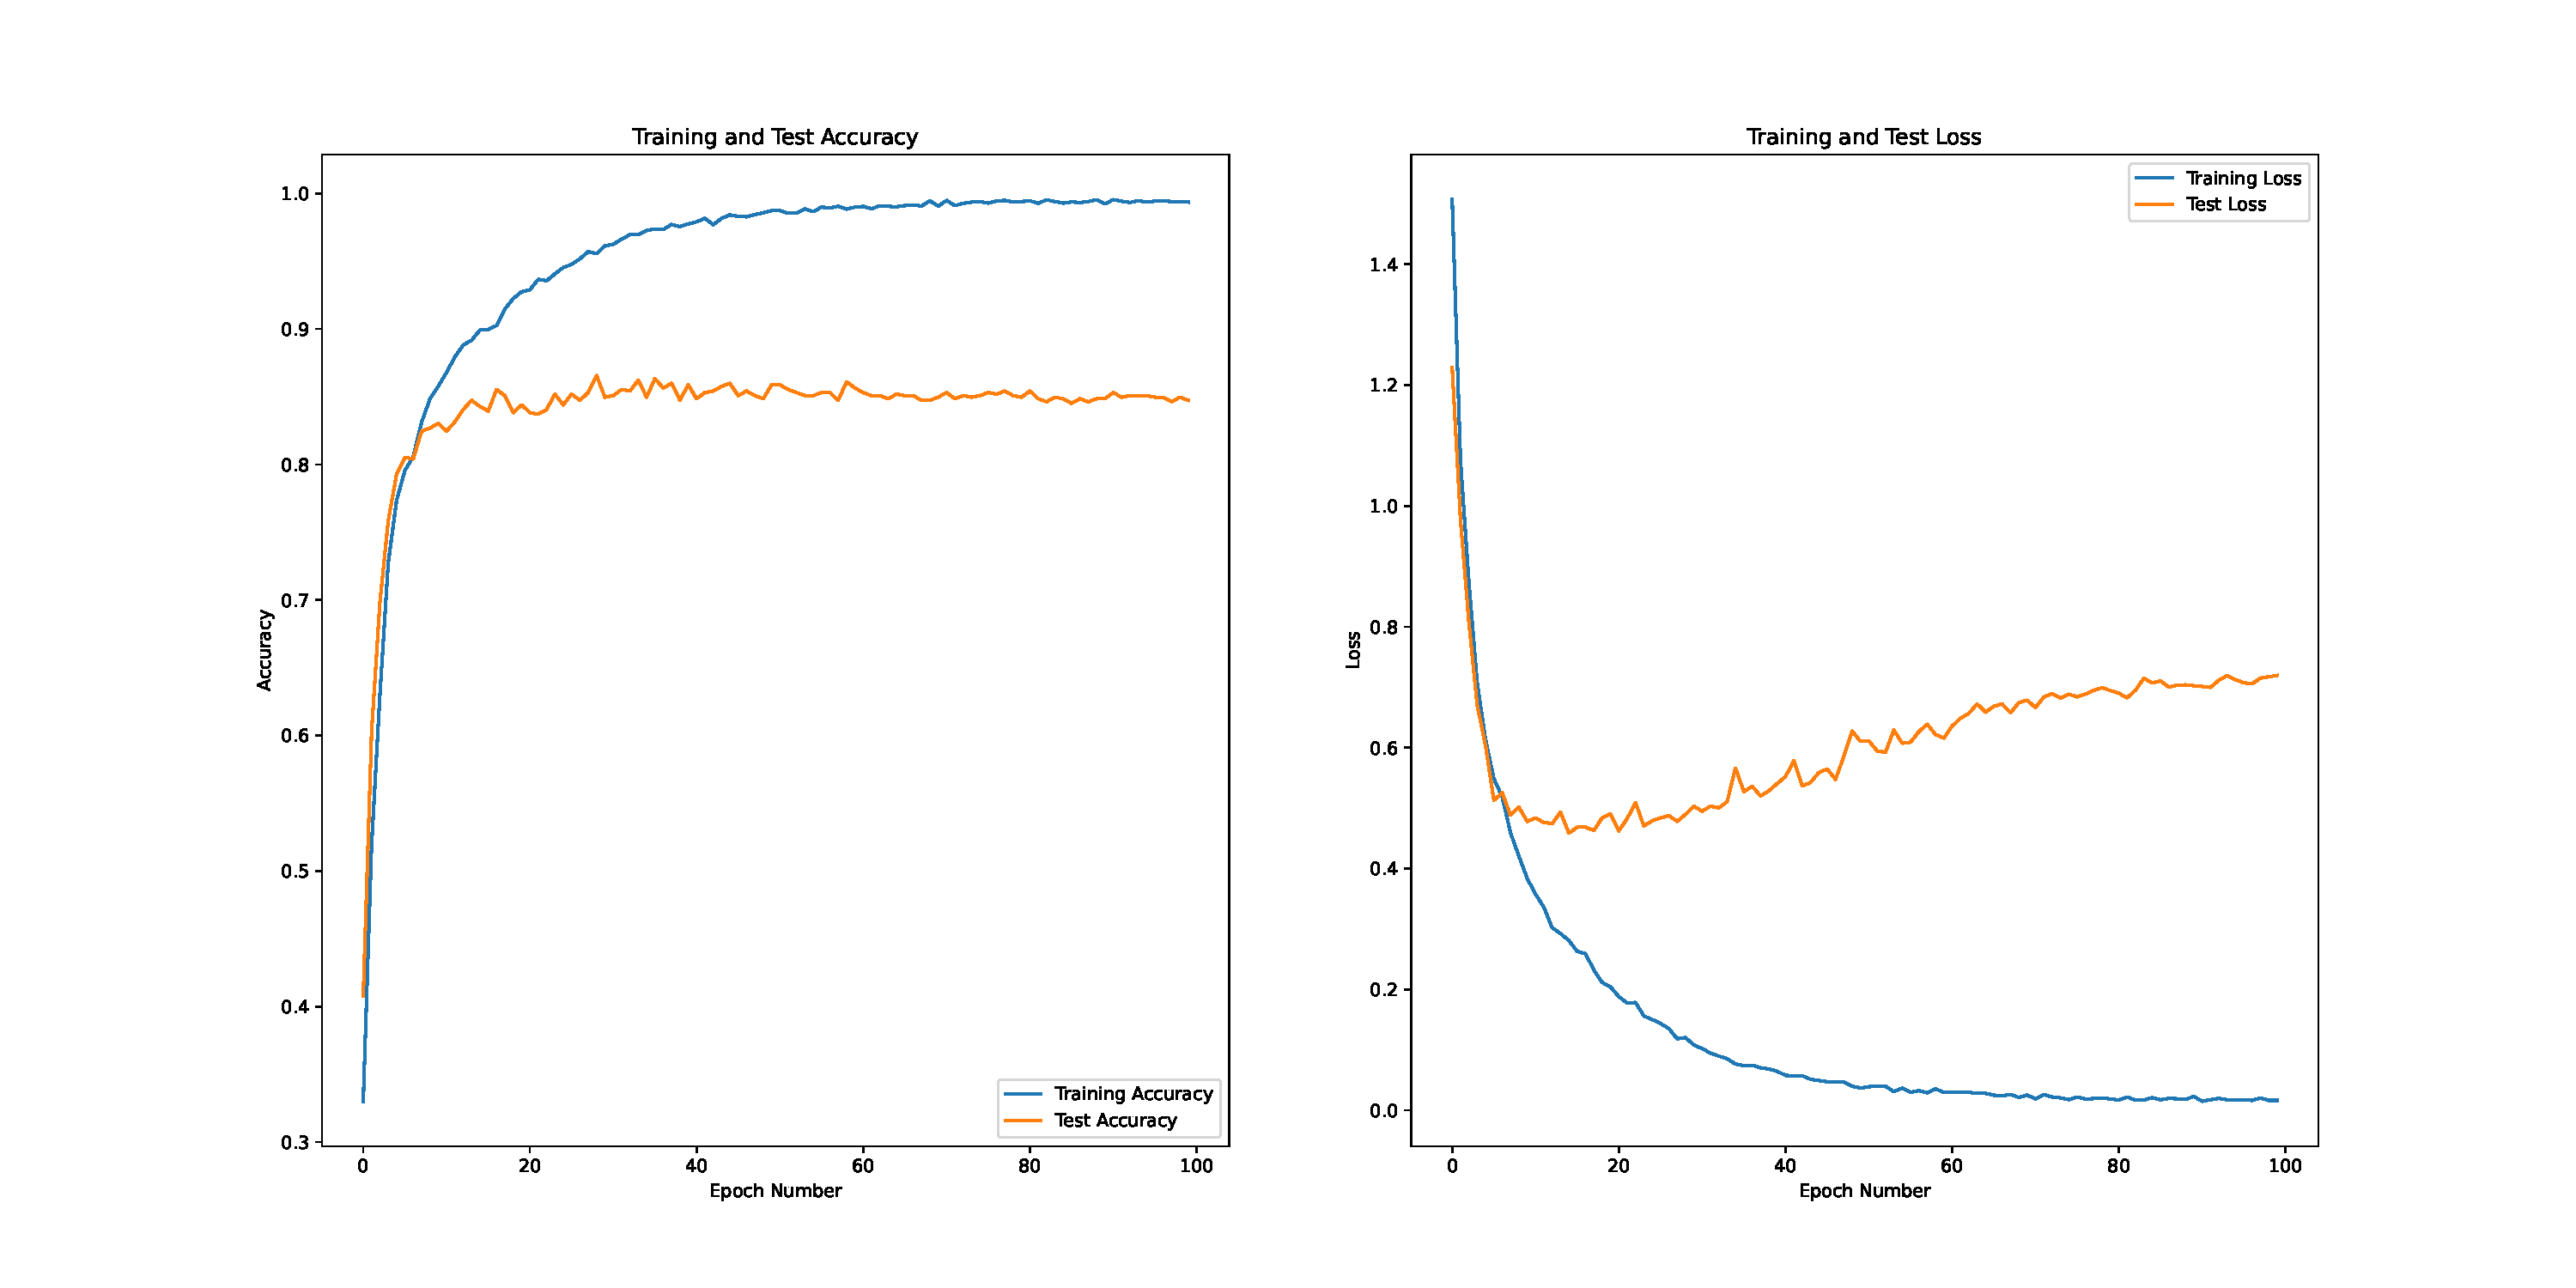
\includegraphics[width=1\textwidth]{metrics/8 metrics.pdf}
\caption{Experiment 8 results}
\label{fig:8 results}
\end{figure}
\begin{table}
\centering
\begin{tabular}{|c|c|c|c|} 
 \hline
 Experiment &  Testing Accuracy & Testing Loss & \acrshort{wer} \\ [0.2ex] 
 \hline
 8 & \accuracyeight & \losseight & \wereight\\
 \hline
\end{tabular}
\caption{The testing accuracy, loss and \acrshort{wer} for experiment 8.}
\label{table: 8 results}
\end{table}
As depicted in Figure~\ref{fig:8 results} and Table~\ref{table: 8 results}, this model architecture produced one of the best performances for lip reading yet. Utilising both landmark and visual features with this \gls{transformer} architecture provides another, different solution for lip reading.\\
The performance of this model was not as good as experiment 5.4 and so further experimentation was carried out.
\section{Experiment 9: CTC Loss}
\label{sec: Experiment 9}
% Experiment 13a,b,c
% CTC loss: 
% Same architecture but different loss measure
\subsection{Model Architecture}
For this experiment, the same model architecture was used as experiment 8, however, the classes and loss metric were changed.\\
Outlined in Section~\ref{sec: CTC Loss}, \acrshort{ctc} loss is a useful loss metric capable of drawing connections between two sequences when this alignment is unknown~\cite{exploration-of-CTC-acoustic-models}. This fits the task of aligning a set of letters, \gls{phoneme}s or \gls{viseme}s to a sequence of video frames.\\
This experiment focused on experimenting with \acrshort{ctc} loss to make three different models capable of predicting the letter, \gls{phoneme} and \gls{viseme} uttered in each frame.\\
Because a different loss metric has been used to train these models, they cannot be directly compared to the previous experiments. Different loss metrics mean that we must independently inspect these models and their performance with lip reading.\\
Different class labels were used for these experiments, changing from \gls{single-label} to \gls{multi-label}. For experiment 9.1 these were the letters for the word uttered, experiment 9.2 used the \gls{phoneme}s and experiment 9.3 used the \gls{viseme}s. This transformed the classes from 1D \gls{one_hot_encoding}s to instead 1D vectors of class numbers.\\
The same \acrshort{lr} scheduling method was used as in experiment 5.5.
\subsection{Results and Evaluation}
\begin{figure}
\centering
    \subfloat[\centering Letter based model]{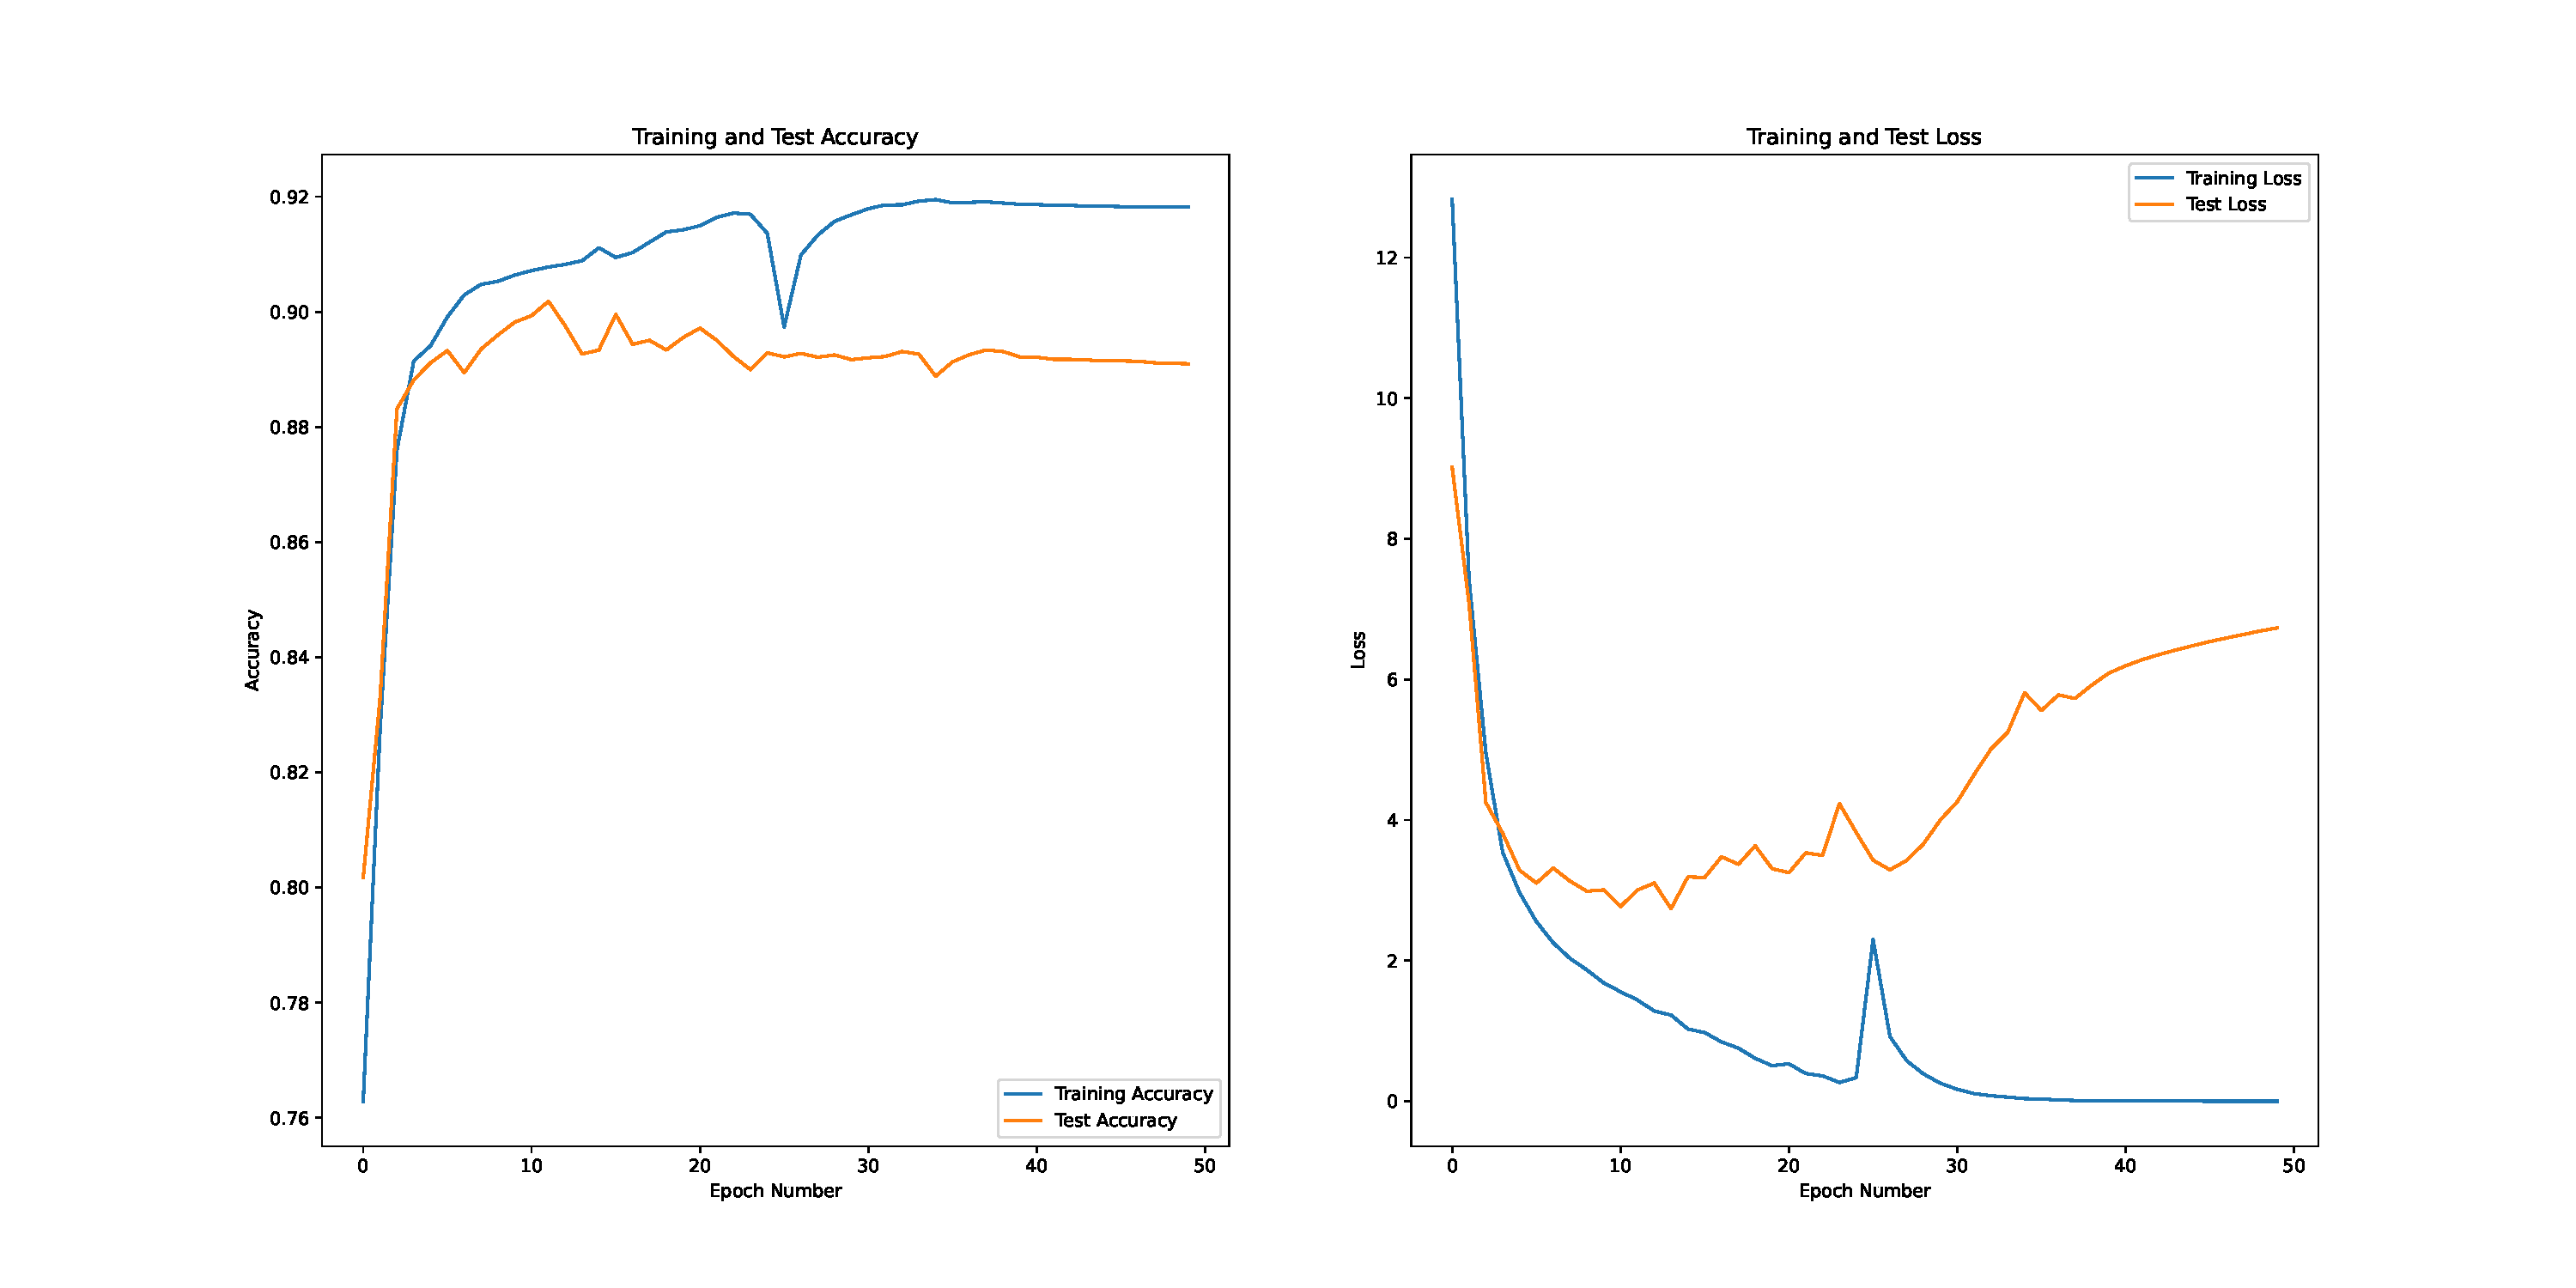
\includegraphics[width=0.5\textwidth]{metrics/9.1 metrics.pdf}}
    \subfloat[\centering \Gls{phoneme} based model]{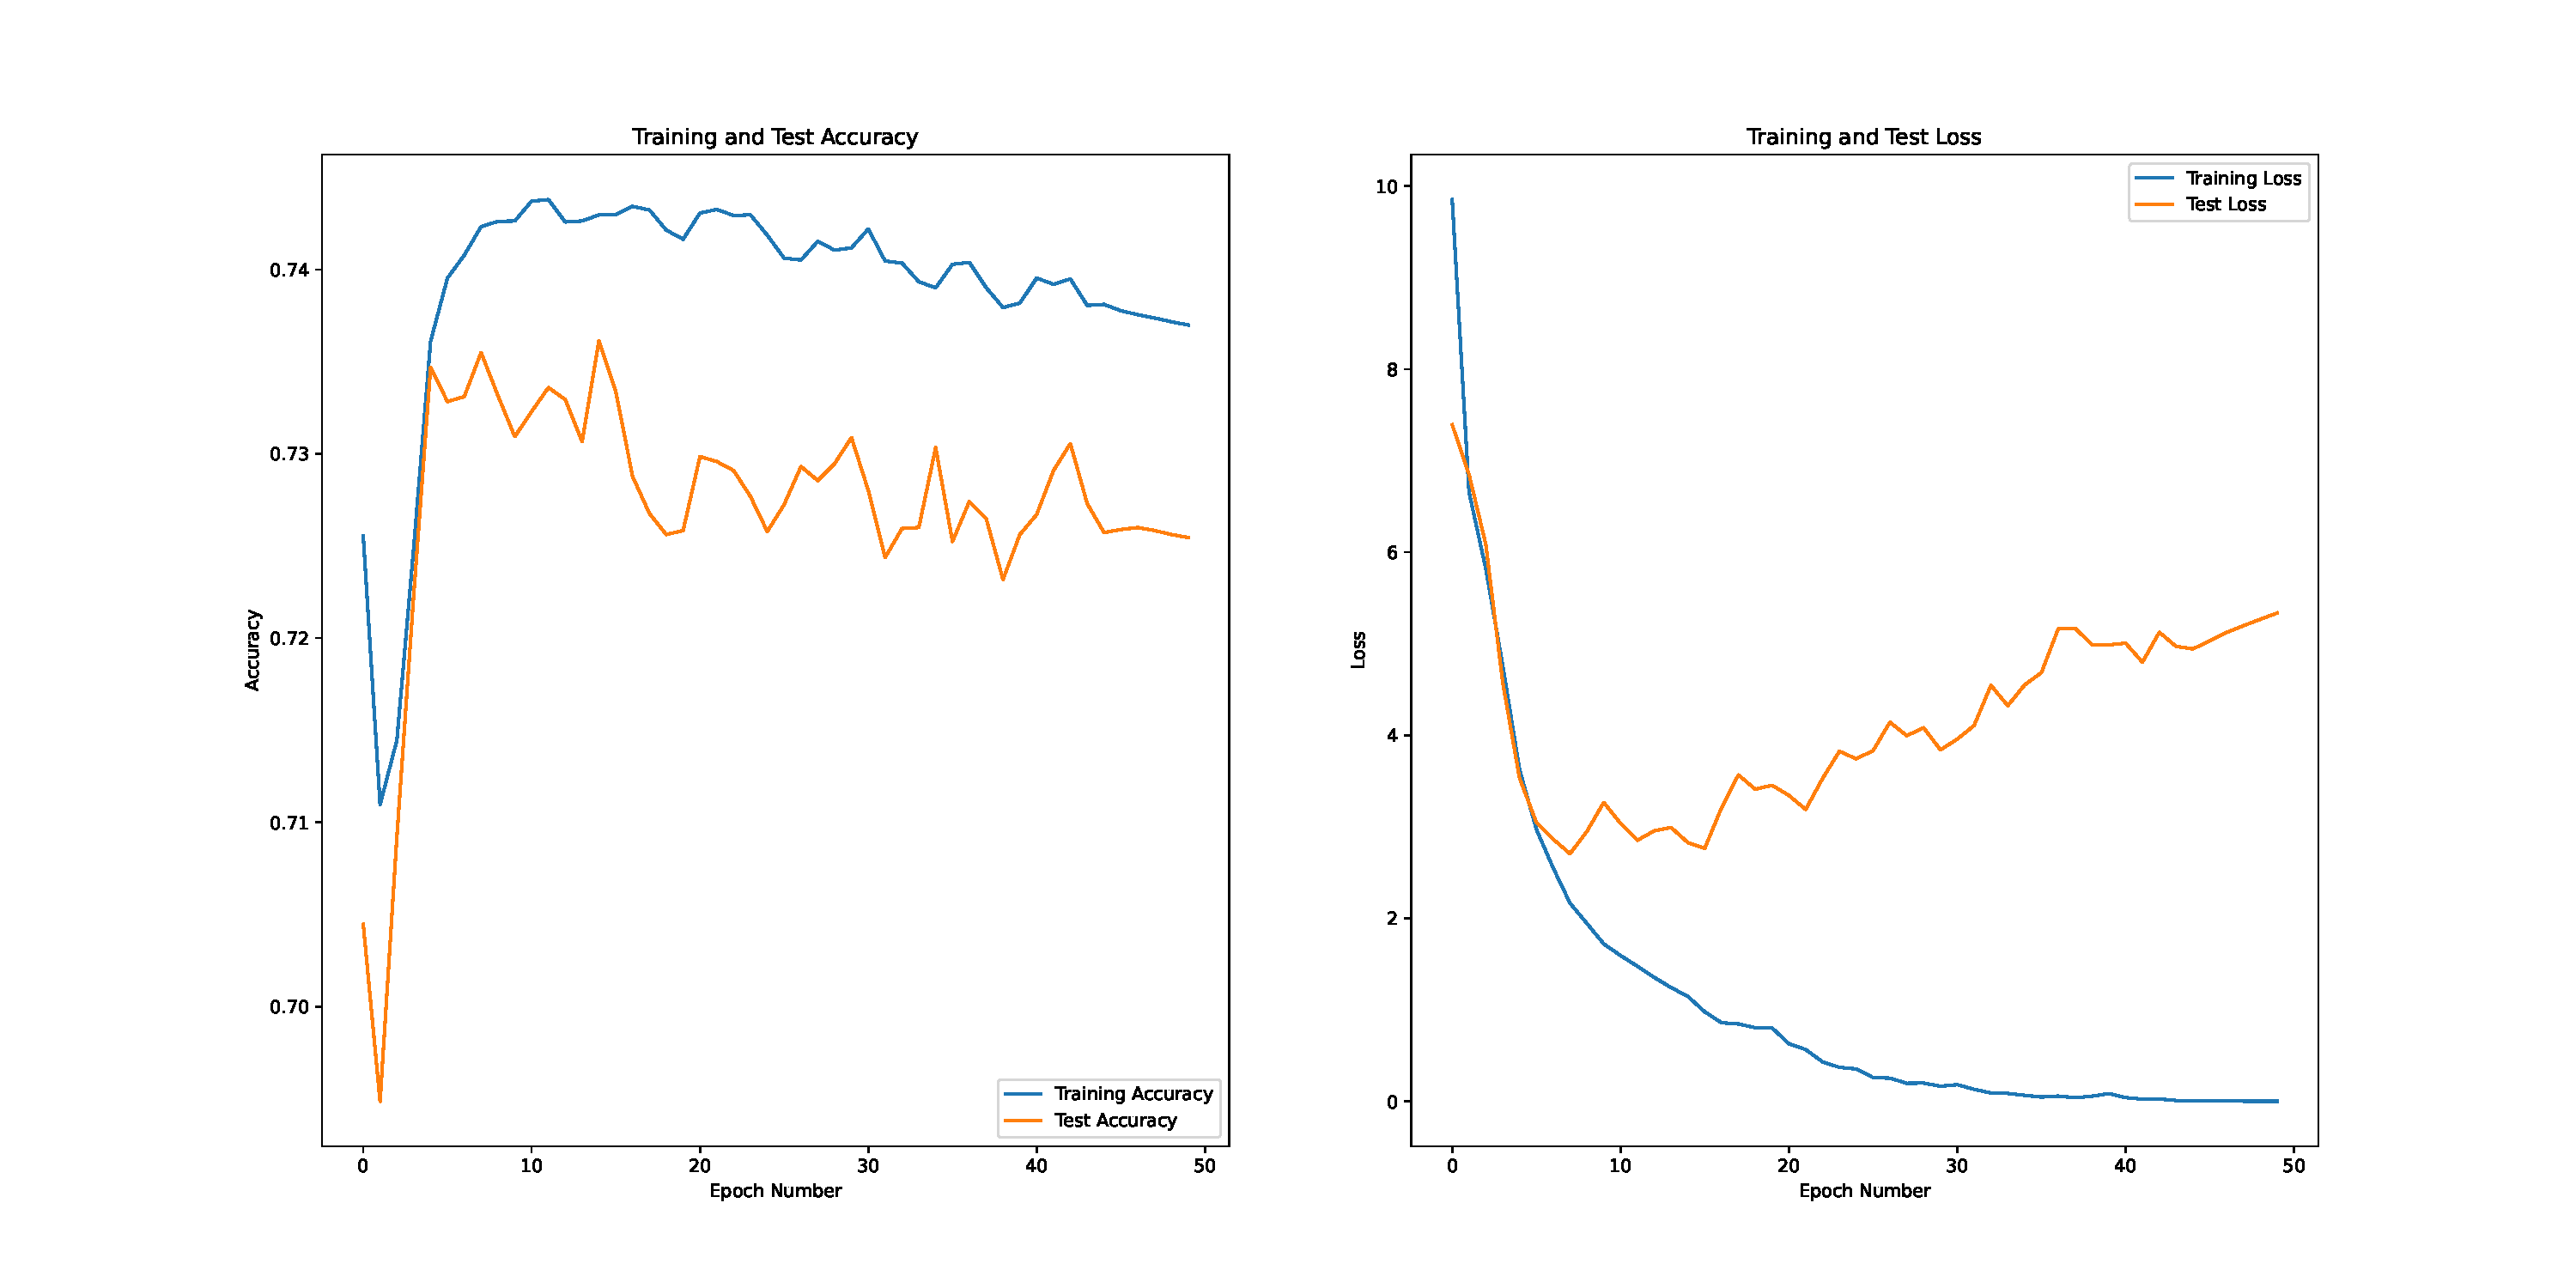
\includegraphics[width=0.5\textwidth]{metrics/9.2 metrics.pdf}}\\
    \subfloat[\centering\Gls{viseme} based model]{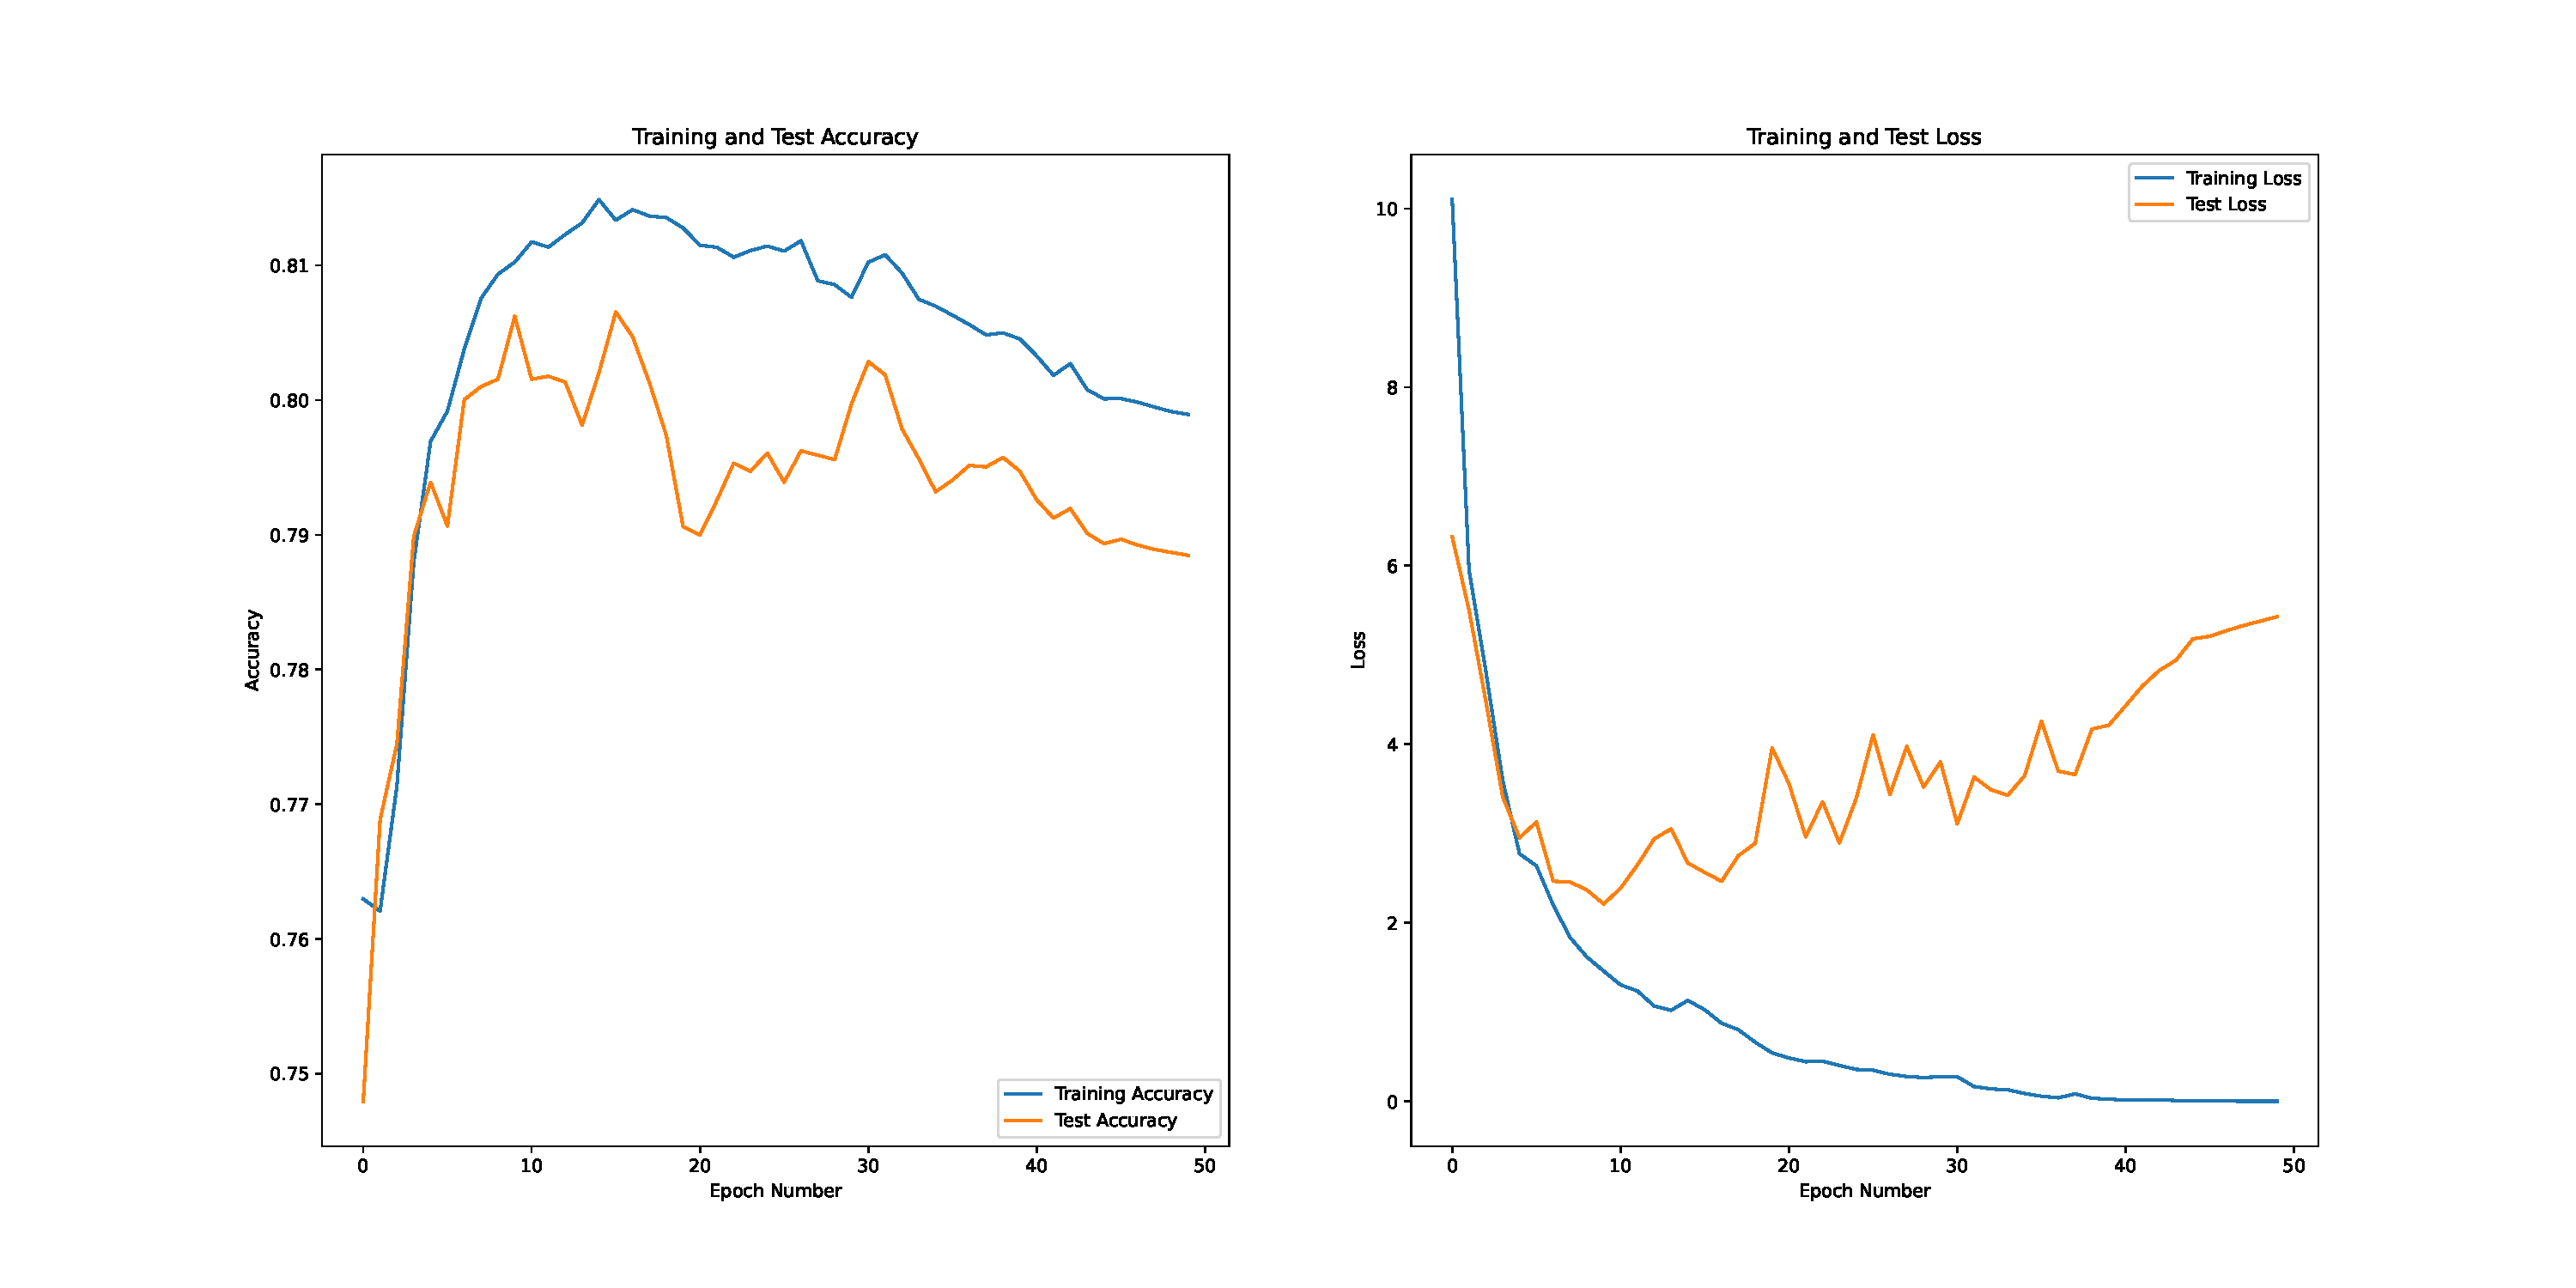
\includegraphics[width=0.5\textwidth]{metrics/9.3 metrics.pdf}}
\caption[Experiment 9 results]{Experiment 9 results. Three different sub-experiments were conducted, using \acrshort{ctc} loss, to compare using the letters, \gls{phoneme}s and \gls{viseme}s as classes for lip reading.}
\label{fig:9 results}
\end{figure}
\begin{table}
\centering
\begin{tabular}{|c|c|c|c|c|} 
 \hline
 Experiment & Class Types &  Testing Accuracy & Testing Loss & \acrshort{wer} \\ [0.2ex] 
 \hline
 9.1 & Letter & \accuracynineone & \lossnineone & \wernineone \\
 9.2 & \Gls{phoneme} & \accuracyninetwo & \lossninetwo & \werninetwo \\
 9.3 &\Gls{viseme} & \accuracyninethree & \lossninethree & \werninethree \\
 \hline
\end{tabular}
\caption[The testing accuracy, loss and \acrshort{wer} for experiment 9]{The testing accuracy, loss and \acrshort{wer} for experiment 9. Three different sub-experiments were conducted, using \acrshort{ctc} loss, to compare using the letters, \gls{phoneme}s and \gls{viseme}s as classes for lip reading.}
\label{table: 9 results}
\end{table}
The findings of this experiment, presented within Table~\ref{table: 9 results} and Figure~\ref{fig:9 results}, are incredibly interesting. As suspected, the best class for lip reading was indeed \gls{viseme}-based, followed by \gls{phoneme}-based and finally letter-based. This is intuitive as many letters in the English language are not pronounced or are pronounced differently depending on the context. For example, the ``h" in ``her" and ``there" are very different.\\
\Gls{phoneme}-based lip reading presented the worst accuracy but better loss and \acrshort{wer} compared with the other methods. A potential reason for this may be some \gls{phoneme}s not being visually represented. Especially in the English lexicon, many sounds are spoken quickly, skipped or pronounced without changes to the facial position. Consequently, the model may struggle to distinguish some words based on their \gls{phoneme}s.\\
The finding that \gls{viseme}-based learning is useful for lip reading is incredibly important and shows the impact of focusing on visual aspects of speech. Furthermore, this proof of concept shows that many visual-only lip reading systems could be improved and made more generic and able to process far more words by looking at their sub-words, particularly their \gls{viseme}s.\\